\documentclass[10pt,a4paper]{report}

% use the packages I need:
\usepackage[english]{babel}             
\usepackage{amsmath}                   
\usepackage{amssymb}                     
\usepackage{epsfig} 
\usepackage{parskip}
\usepackage{booktabs}
\usepackage{gensymb}
\usepackage{graphicx} 
\usepackage{placeins}
\usepackage{caption}
\usepackage{subcaption}
\usepackage{inputenc}
\usepackage{braket} 
\usepackage{slashed} 
\usepackage{pdfpages}
\usepackage{enumitem} 

% Define code listings:
\usepackage{listings}
\lstset {
    language=C++,
    backgroundcolor=\color{black!5}, % set backgroundcolor
    basicstyle=\footnotesize,% basic font setting
}

% Define our own chapter titles:
\usepackage{titlesec}
\titleformat{\chapter}[hang]{\normalfont\raggedright\Huge\bfseries}{\thechapter ~~}{0pt}{\Huge}
\titlespacing*{\chapter}{0pt}{-40pt}{20pt}
\titlespacing*{\section}{0pt}{15pt}{0pt}
\titlespacing*{\subsection}{0pt}{5pt}{0pt}

% Define your own paper size:
\usepackage{geometry}
%\geometry{papersize={170.0mm,240.0mm}} % absolute paper size.
\geometry{papersize={204.0mm,290.0mm}} % absolute paper size.
\geometry{top=10.0mm}                  % Top marging.
\geometry{bottom=10.0mm}               % Bottom margin.
\geometry{left=10.0mm}                 % Left margin.
\geometry{right=10.0mm}                % Right margin. 

% new commands:
\newcommand{\elmt}[2]{${^{#2} \textrm{#1}}$}
\newcommand{\elmnt}[3]{${^{#2} \textrm{#1} ^{#3}}$}
\newcommand{\elmf}[2]{^{#2} \textrm{#1}}
\newcommand{\elmnf}[3]{^{#2} \textrm{#1} ^{#3}}
\newcommand{\MeV}[0]{\ \textrm{MeV}}
\newcommand{\AMeV}[0]{\ \textrm{MeV/u}}
\newcommand{\keV}[0]{\ \textrm{keV}}
\newcommand{\AkeV}[0]{\ \textrm{keV/u}}
\newcommand{\GeV}[0]{\ \textrm{GeV}}
\newcommand{\AGeV}[0]{\ \textrm{GeV/u}}
\newcommand{\eV}[0]{\ \textrm{eV}}
\newcommand{\AeV}[0]{\ \textrm{eV/u}}
\newcommand{\mgcm}[0]{\ \textrm{mg} / \textrm{cm} ^{2}}
\newcommand{\Het}[0]{${( ^{3} \textrm{He}, t) \ }$}
\newcommand{\rtb}[0]{${\textrm{R} ^{3} \textrm{B}}$ }
\newcommand{\rtbn}[0]{${\textrm{R} ^{3} \textrm{B}}$}
\newcommand{\rtbp}[0]{${\textrm{R} ^{3} \textrm{B}}$}
\newcommand{\rtbe}[0]{${\textrm{R} ^{3} \textrm{B}}$ experiment }
\newcommand{\rtbep}[0]{${\textrm{R} ^{3} \textrm{B}}$ experiment}
\newcommand{\rtbs}[0]{${\textrm{R} ^{3} \textrm{B}}$ setup }
\newcommand{\rtbsp}[0]{${\textrm{R} ^{3} \textrm{B}}$ setup}
\newcommand{\rtbsNL}[0]{${\textrm{R} ^{3} \textrm{B}}$ meetopstelling }
\newcommand{\rtbsNLp}[0]{${\textrm{R} ^{3} \textrm{B}}$ meetopstelling}
\newcommand{\rtbc}[0]{${\textrm{R} ^{3} \textrm{B}}$ collaboration }
\newcommand{\rtbcp}[0]{${\textrm{R} ^{3} \textrm{B}}$ collaboration }
\newcommand{\lrtb}[0]{${\textrm{LAND} - \textrm{R} ^{3} \textrm{B}}$ }
\newcommand{\lrtbp}[0]{${\textrm{LAND} - \textrm{R} ^{3} \textrm{B}}$}
\newcommand{\lrtbs}[0]{${\textrm{LAND}}$-${\textrm{R} ^{3} \textrm{B}}$ setup }
\newcommand{\lrtbsp}[0]{${\textrm{LAND}}$-${\textrm{R} ^{3} \textrm{B}}$ setup}
\newcommand{\rtbroot}[0]{${\textrm{R} ^{3} \textrm{B}}$Root }
\newcommand{\rtbrootp}[0]{${\textrm{R} ^{3} \textrm{B}}$Root}
\newcommand{\rtbf}[0]{\textrm{R} ^{3} \textrm{B}}
\newcommand{\cel}[0]{\ \degree \textrm{C}}
\newcommand{\parincl}{\mathbin{\!/\mkern-5mu/\!}}
\newcommand{\optcoeff}[2]{ ( #1 | #2 ) }
\newcommand{\whitez}[0]{\textcolor{white}{0}}

% Get right fonts of paragraphs:
\setlength{\parindent}{0cm}
\setlength{\parskip}{10pt}
\setlength{\belowcaptionskip}{5pt}
\setlength{\abovecaptionskip}{5pt}

% Manage floats:
\renewcommand{\floatpagefraction}{.8}
%\renewcommand{\topfraction}{.9}
%\renewcommand{\bottomfraction}{.1}
%\renewcommand{\textfraction}{.01}

% Manage our bibliography:
\usepackage[square,comma,numbers,sort&compress]{natbib}
\usepackage{notoccite}
\bibliographystyle{ieeetr} 
\usepackage[nottoc,notlot,notlof]{tocbibind} % Disables inclusion of table of contents, figures, tables in the contents.
\usepackage{tocstyle} % Saves Table of Contents, etc. if this is loaded AFTER notoccite.
\usetocstyle{standard}

% Give input for LaTeX title page:
\title{Measurement of the Gamow Teller states in ${^{116} \textrm{Sb}}$ and ${^{122} \textrm{Sb}}$}
\author{Christiaan Alwin Douma} 

% Start the document:

\begin{document} 

\begin{figure}[htbp]
    \centering
    \begin{subfigure}[htbp]{0.42\textwidth}
        \subcaption{\textbf{Physics List ${=}$ FTFP-INCLXX-HP}}
        \label{fig:A1}
        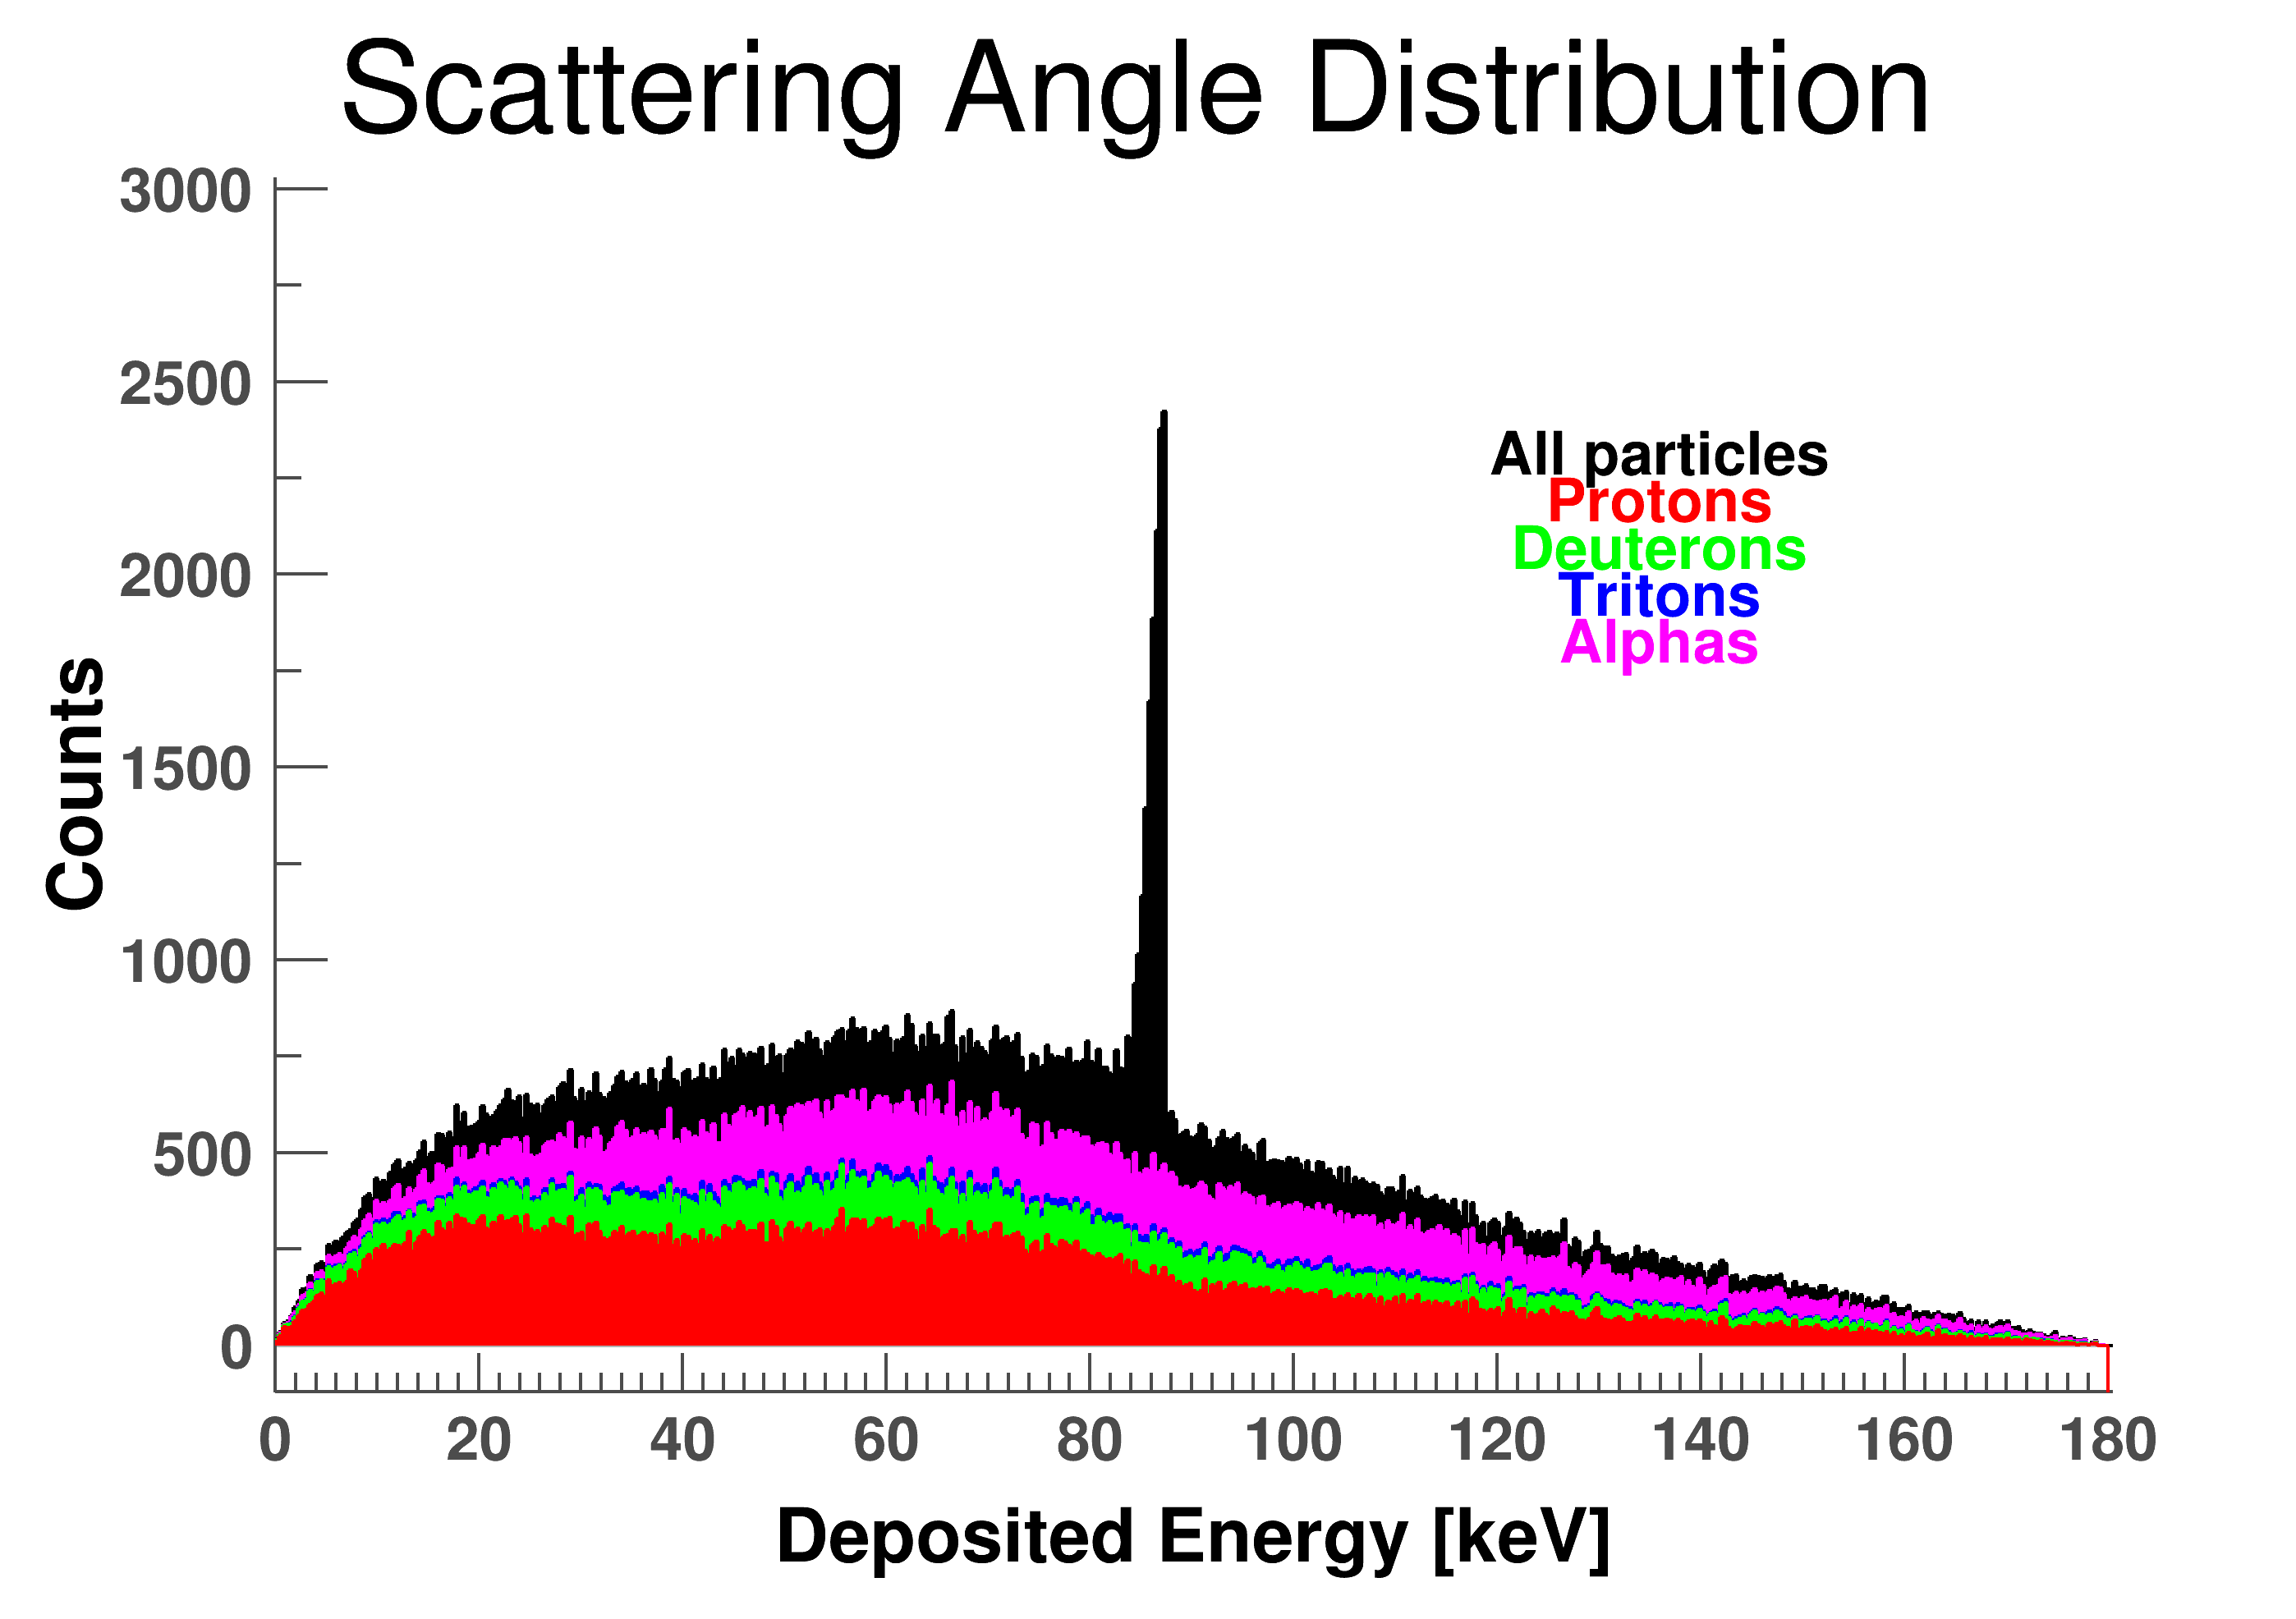
\includegraphics[width=\textwidth]{./A1_FTFP_INCLXX_HP_Scat.png}
    \end{subfigure}
    ~ 
    \begin{subfigure}[htbp]{0.42\textwidth}
        \subcaption{\textbf{Physics List ${=}$ QGSP-INCLXX}}
        \label{fig:A2}
        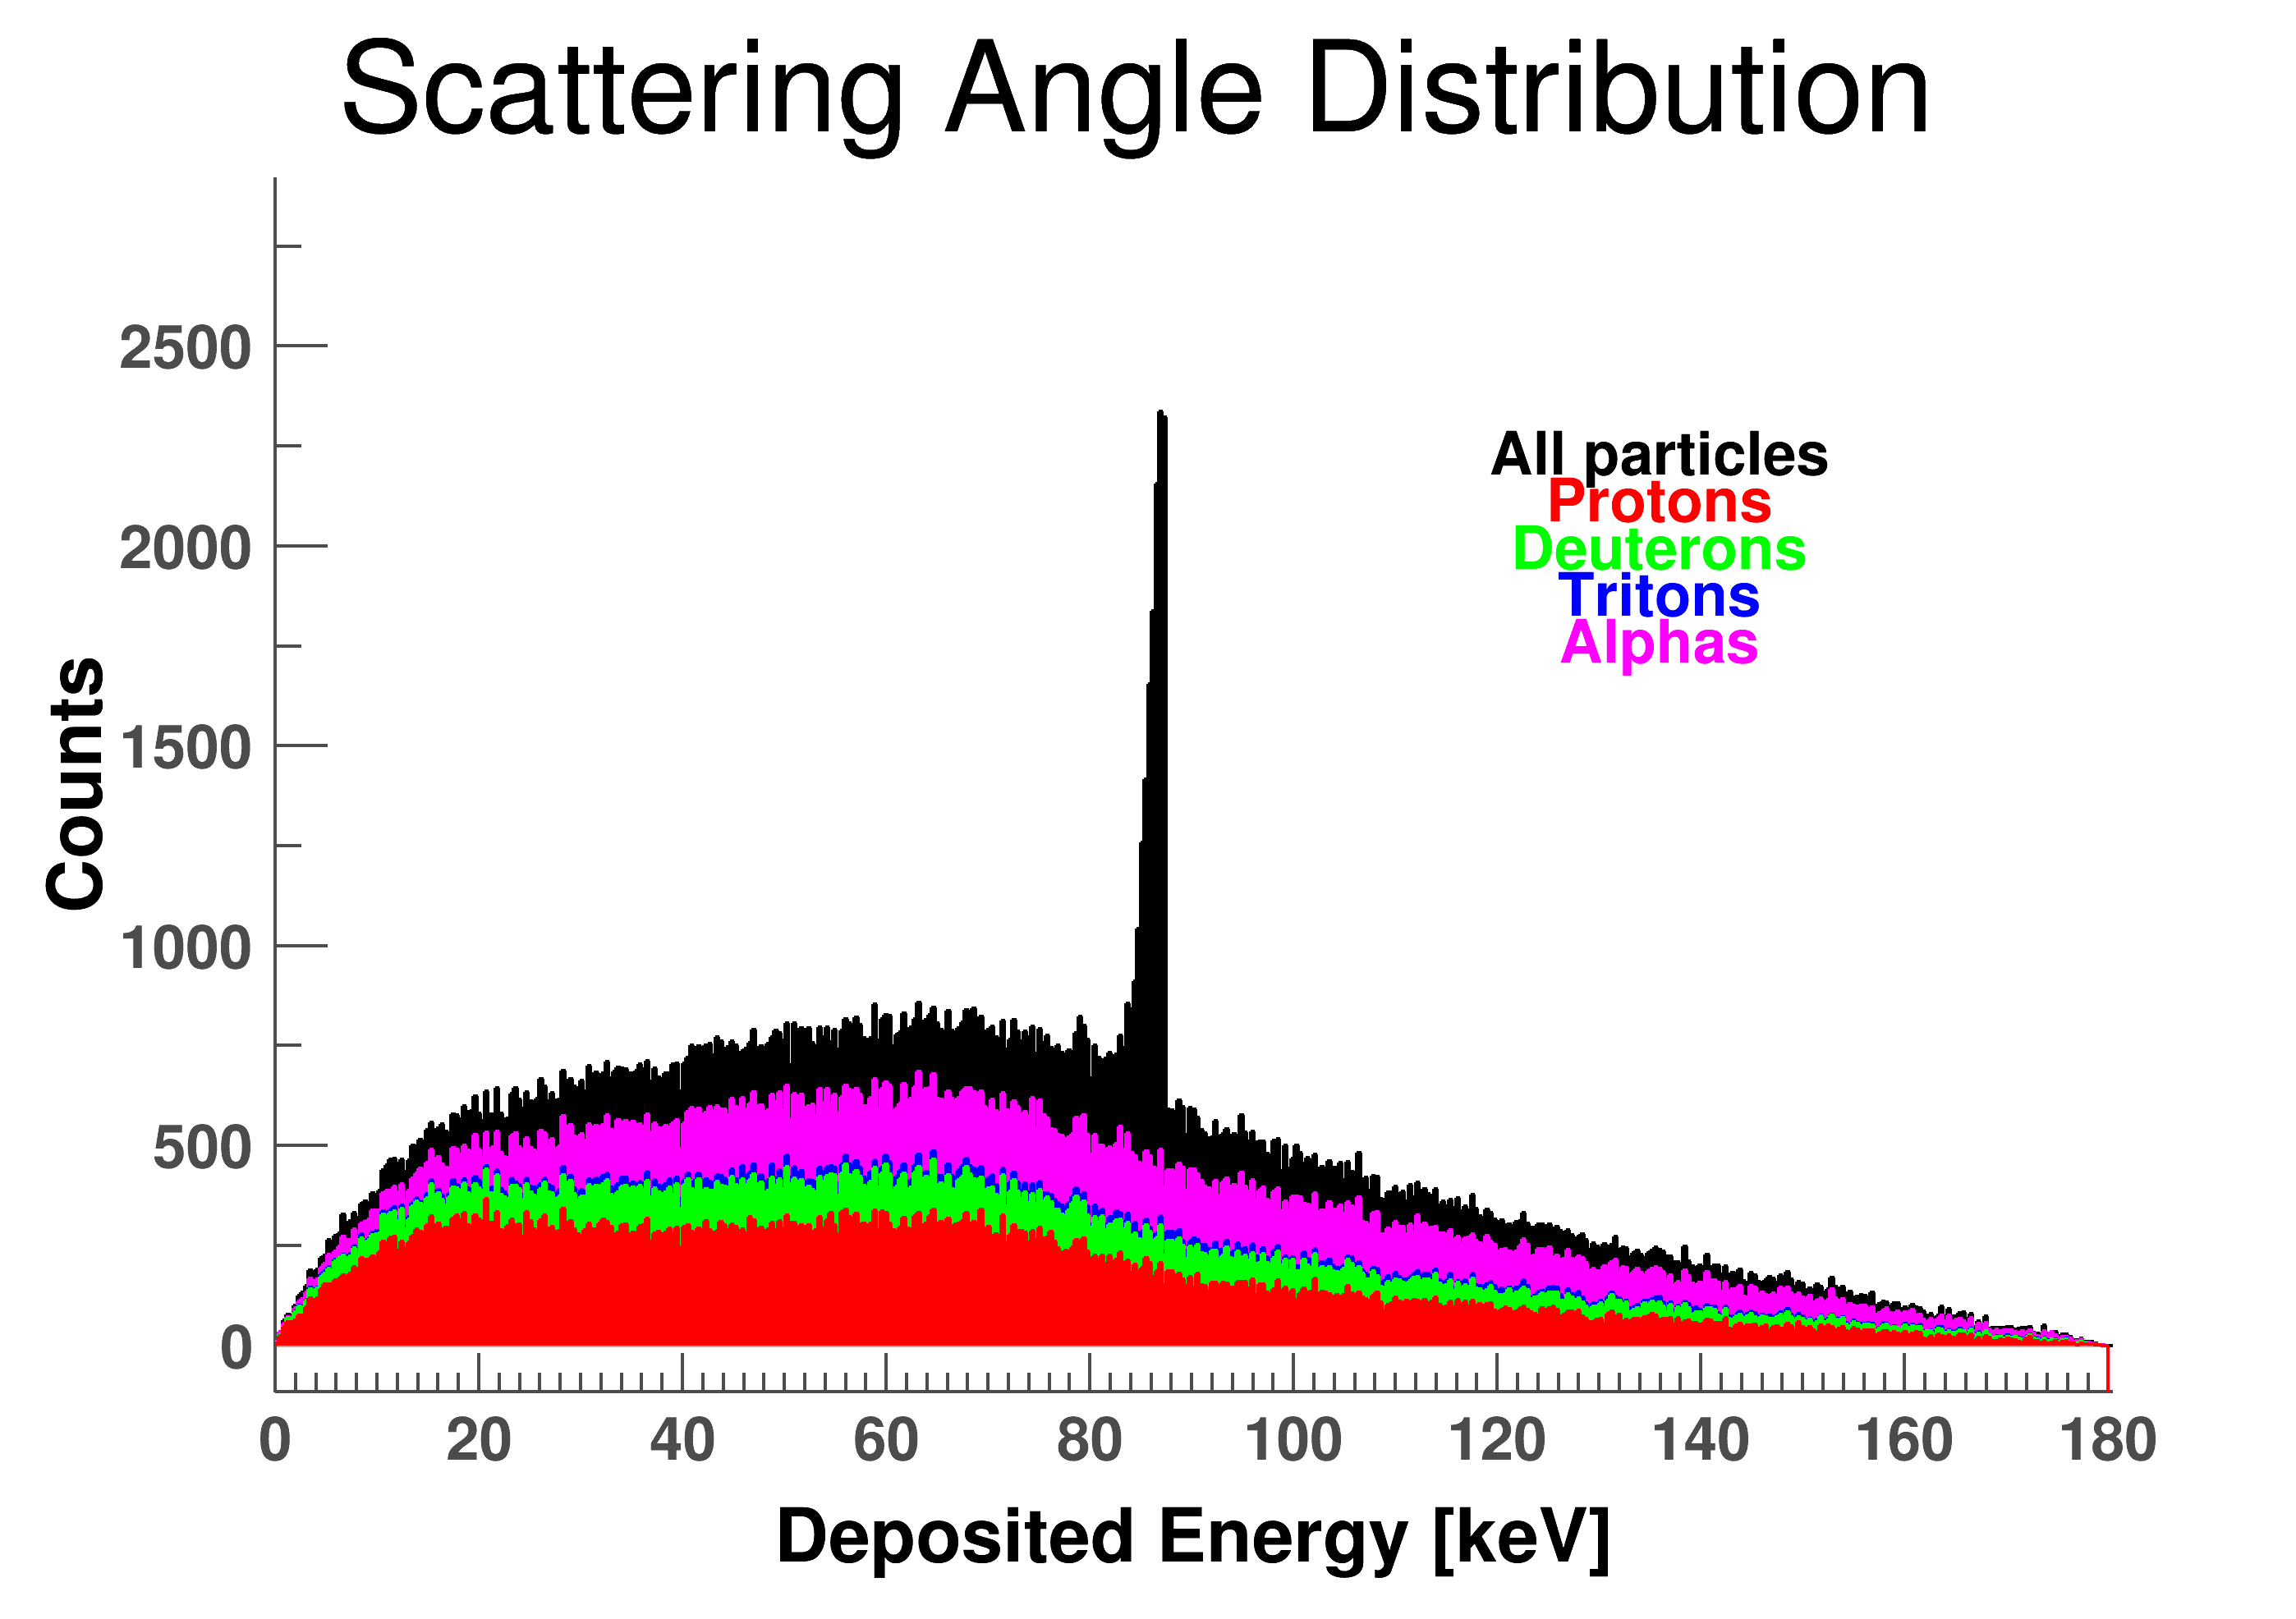
\includegraphics[width=\textwidth]{./A2_QGSP_INCLXX_Scat.png}
    \end{subfigure}
    
    \vspace{1mm}
    
    \begin{subfigure}[htbp]{0.42\textwidth}
        \subcaption{\textbf{Physics List ${=}$ QGSP-INCLXX-HP}}
        \label{fig:A3}
        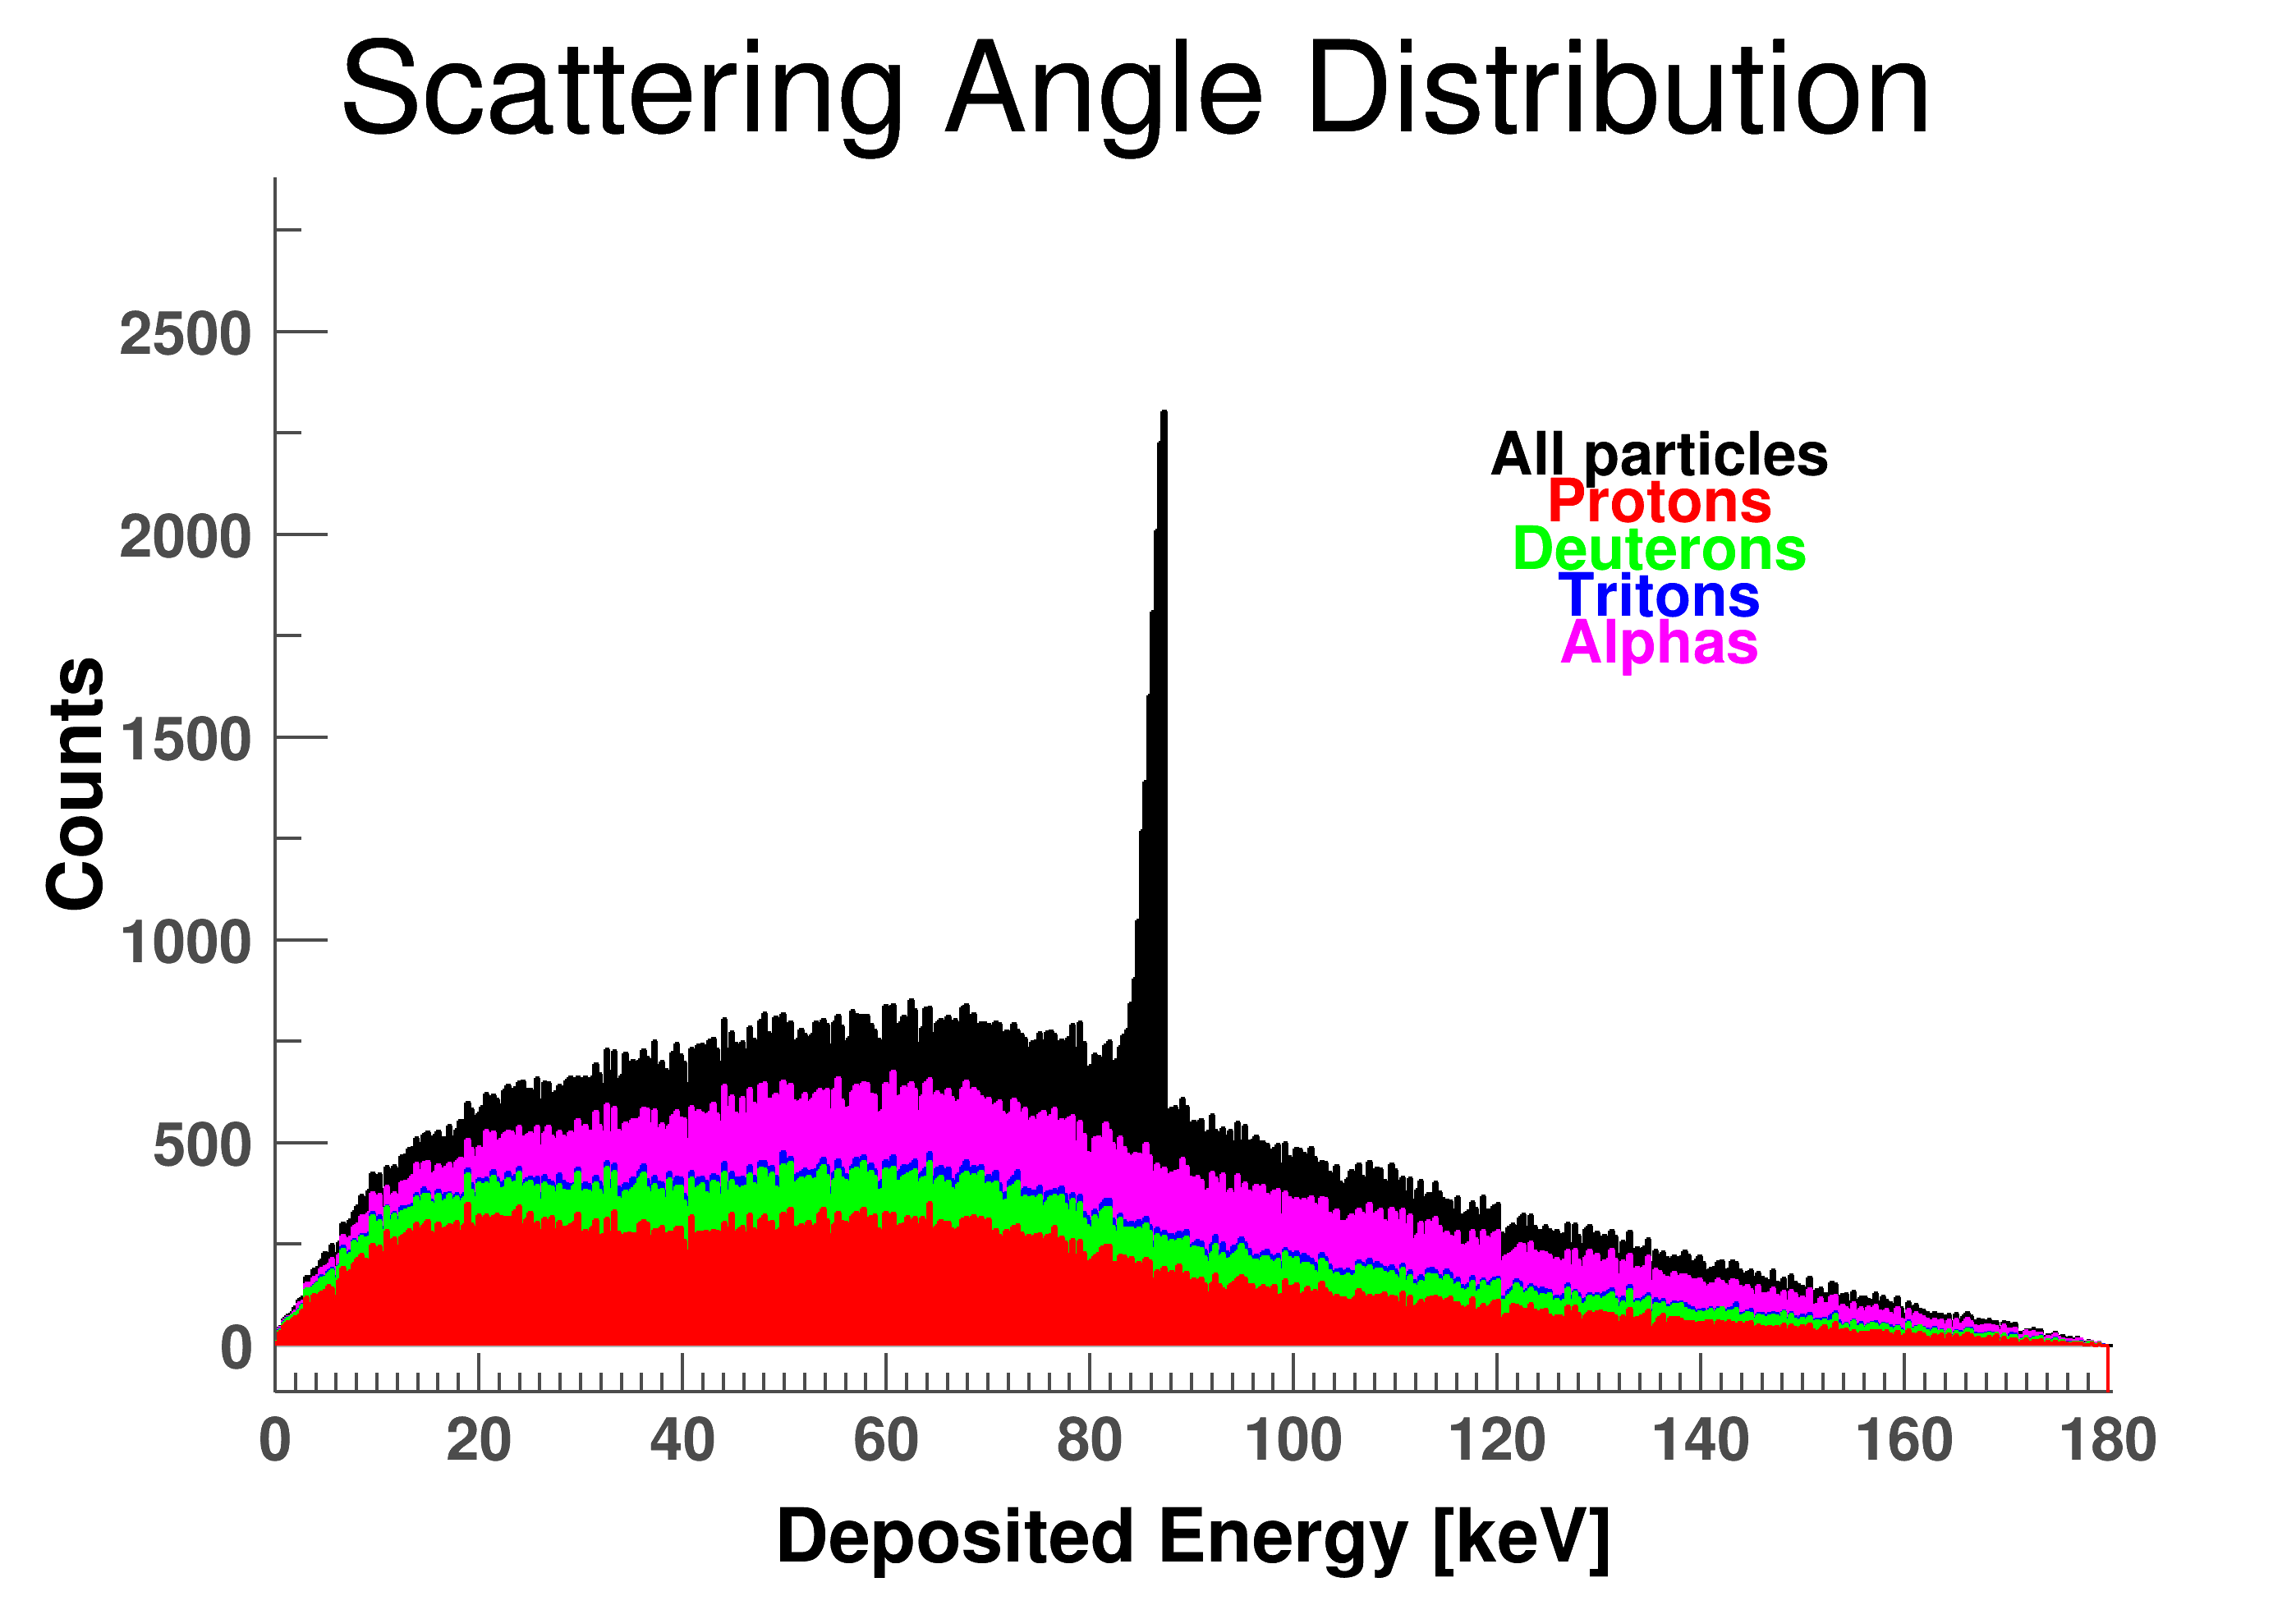
\includegraphics[width=\textwidth]{./A3_QGSP_INCLXX_HP_Scat.png}
    \end{subfigure}
    ~ 
    \begin{subfigure}[htbp]{0.42\textwidth}
        \subcaption{\textbf{Physics List ${=}$ QGSP-BERT-HP}}
        \label{fig:A4}
        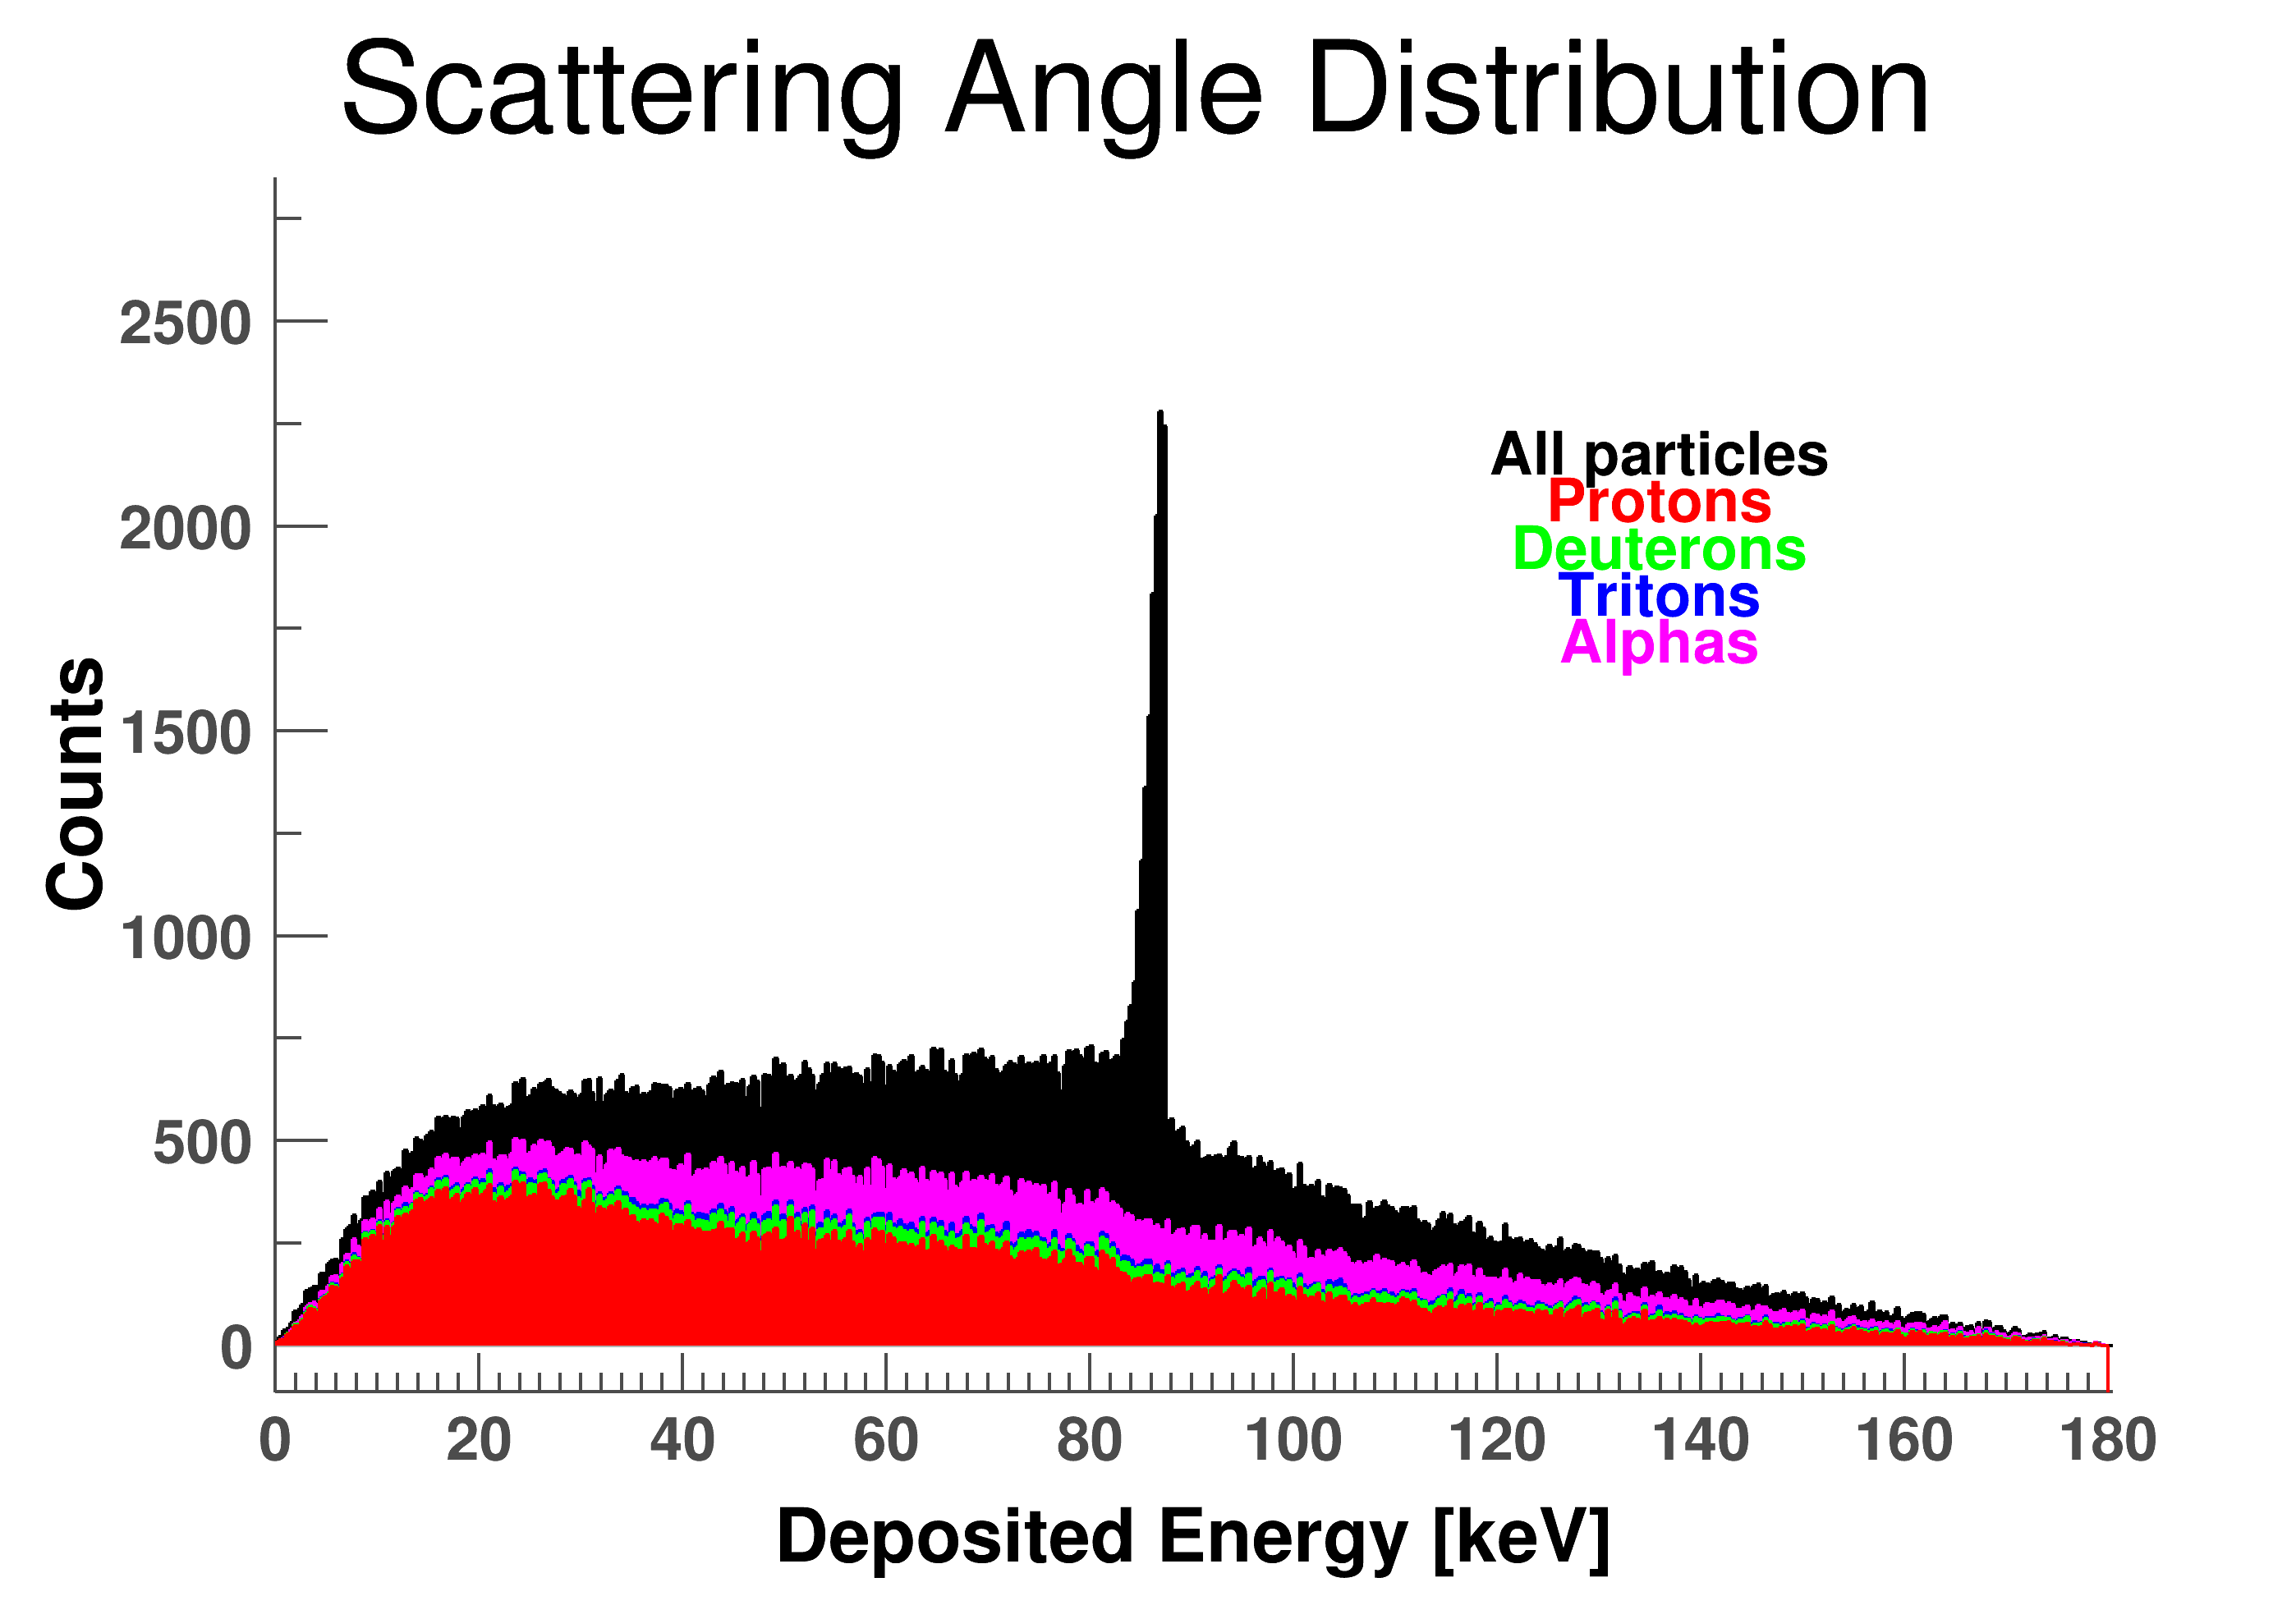
\includegraphics[width=\textwidth]{./A4_QGSP_BERT_HP_Scat.png}
    \end{subfigure}
    
    \vspace{1mm}
    
    \begin{subfigure}[htbp]{0.42\textwidth}
        \subcaption{\textbf{Physics List ${=}$ QGSP-BIC-HP}}
        \label{fig:A5}
        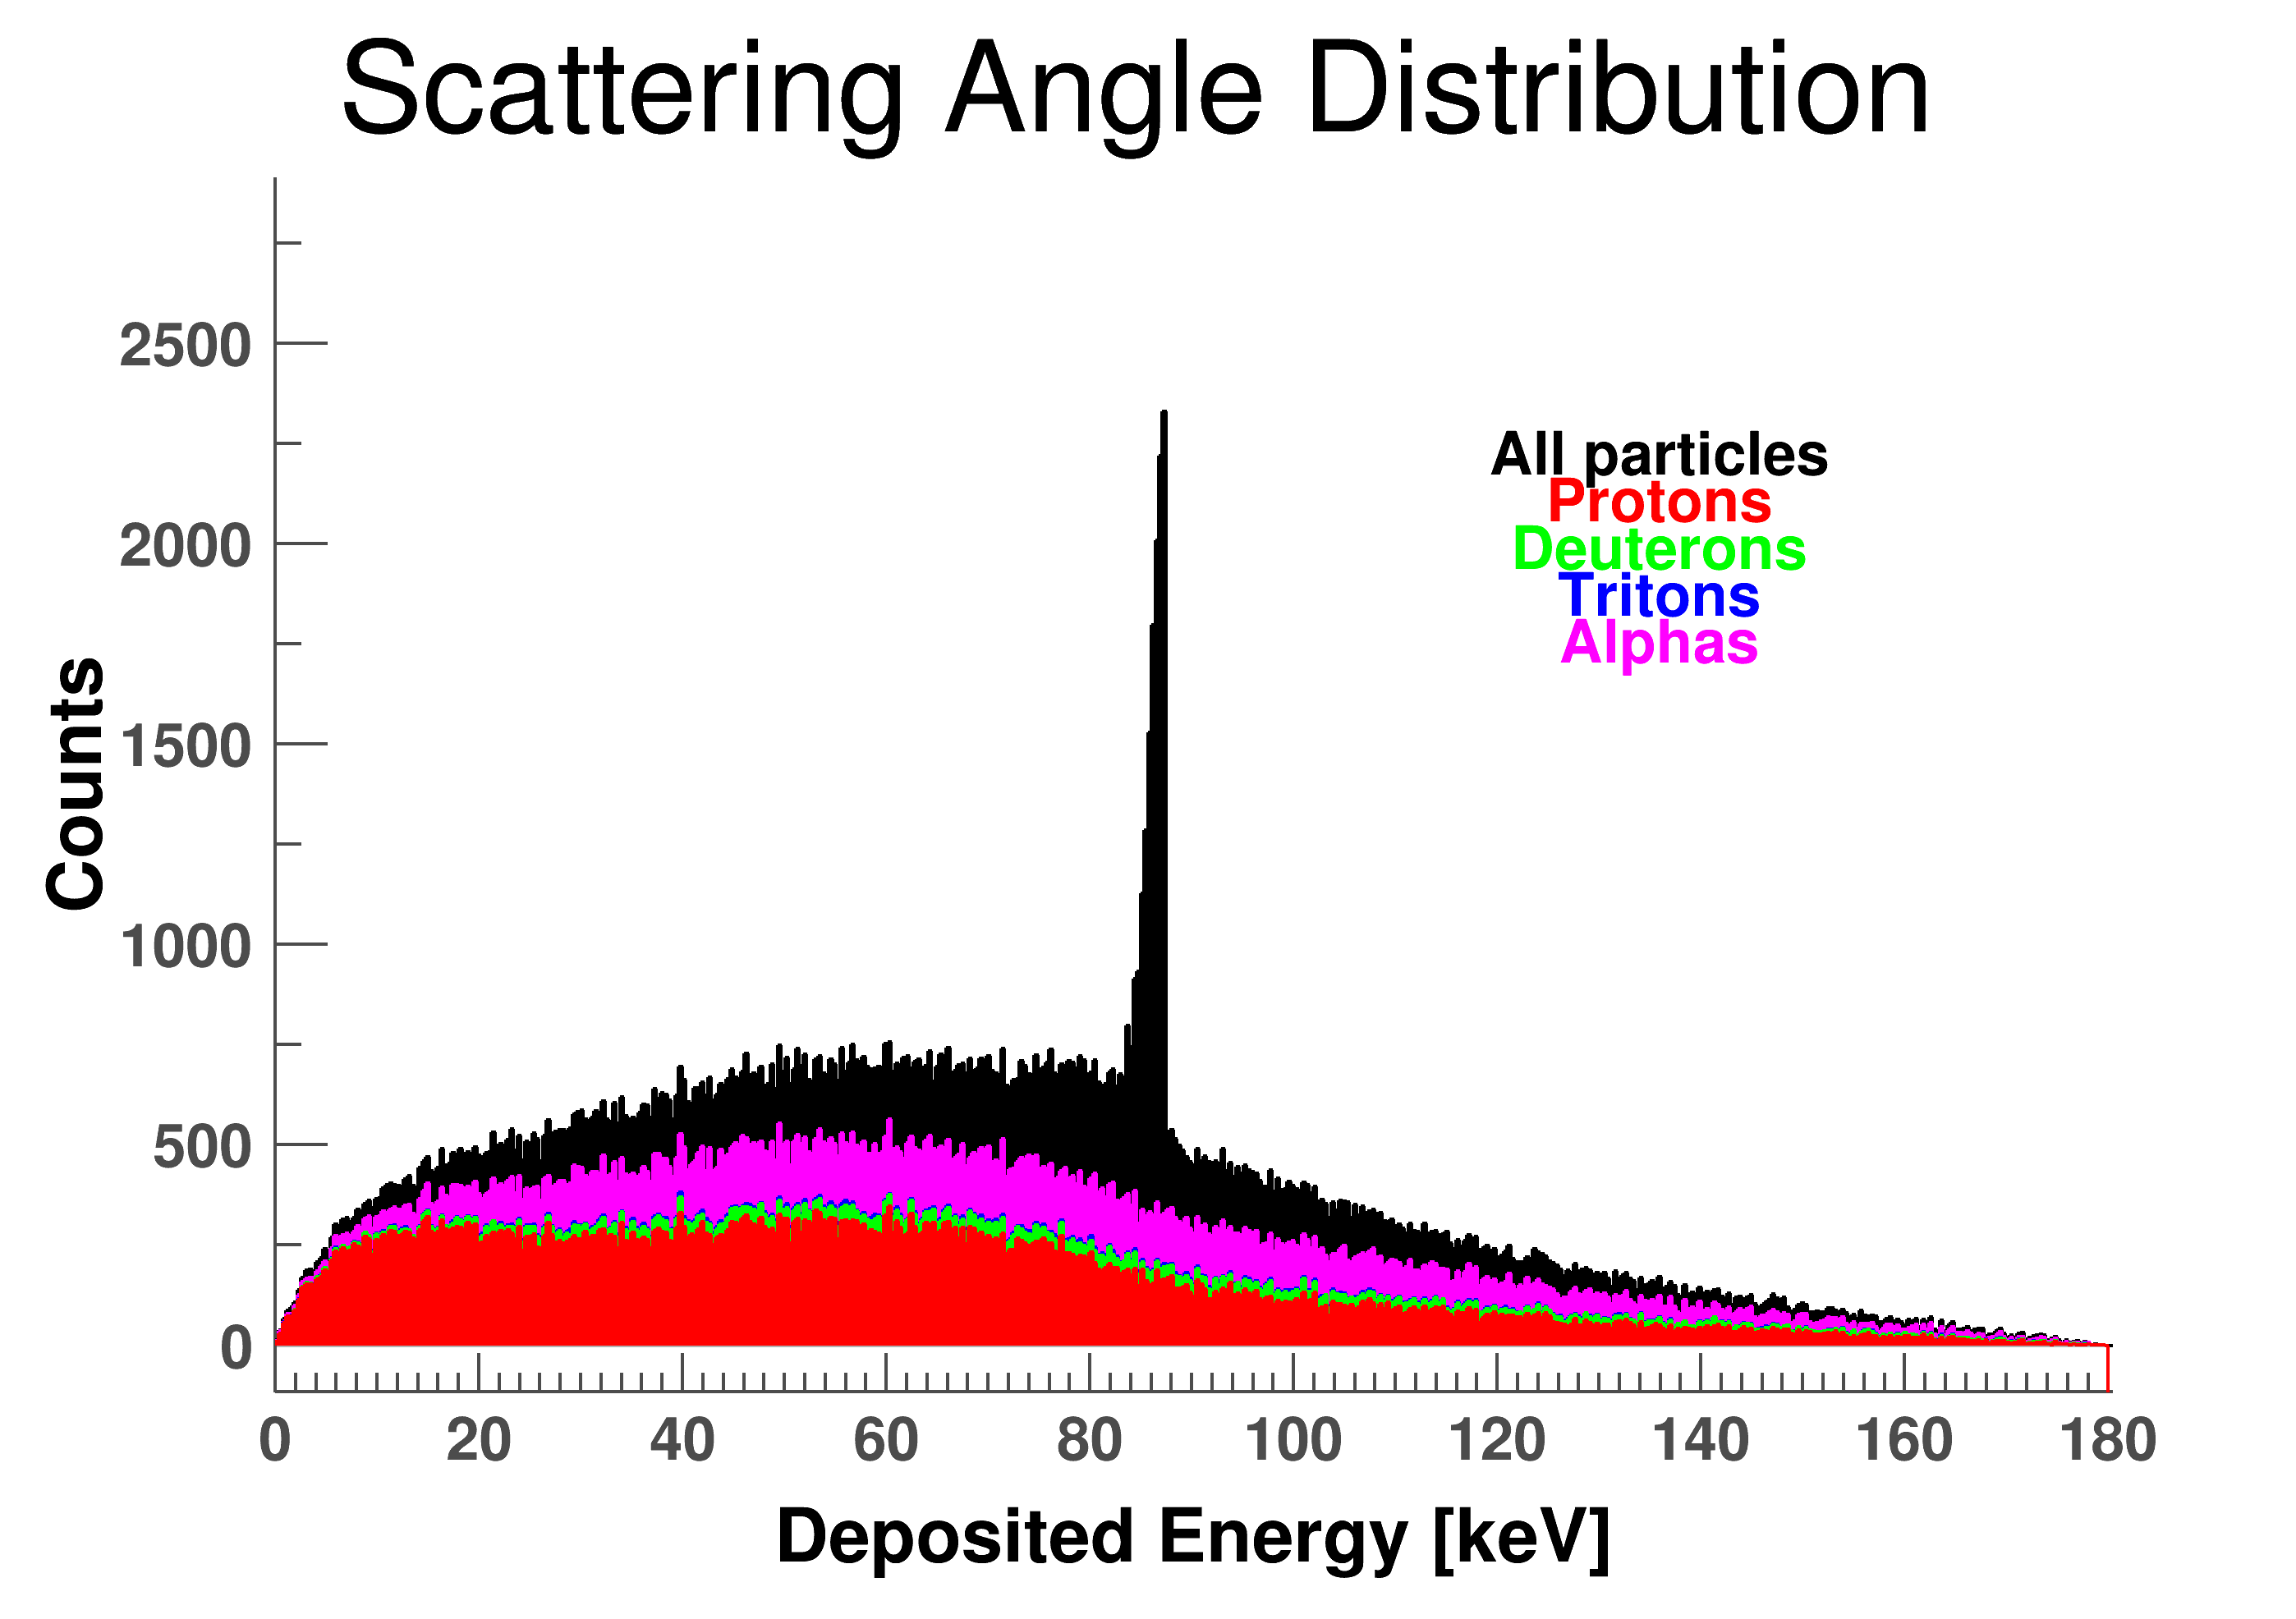
\includegraphics[width=\textwidth]{./A5_QGSP_BIC_HP_Scat.png}
    \end{subfigure}
    ~ 
    \begin{subfigure}[htbp]{0.42\textwidth} 
        \subcaption{\textbf{Physics List ${=}$ QBBC}}
        \label{fig:A6}
        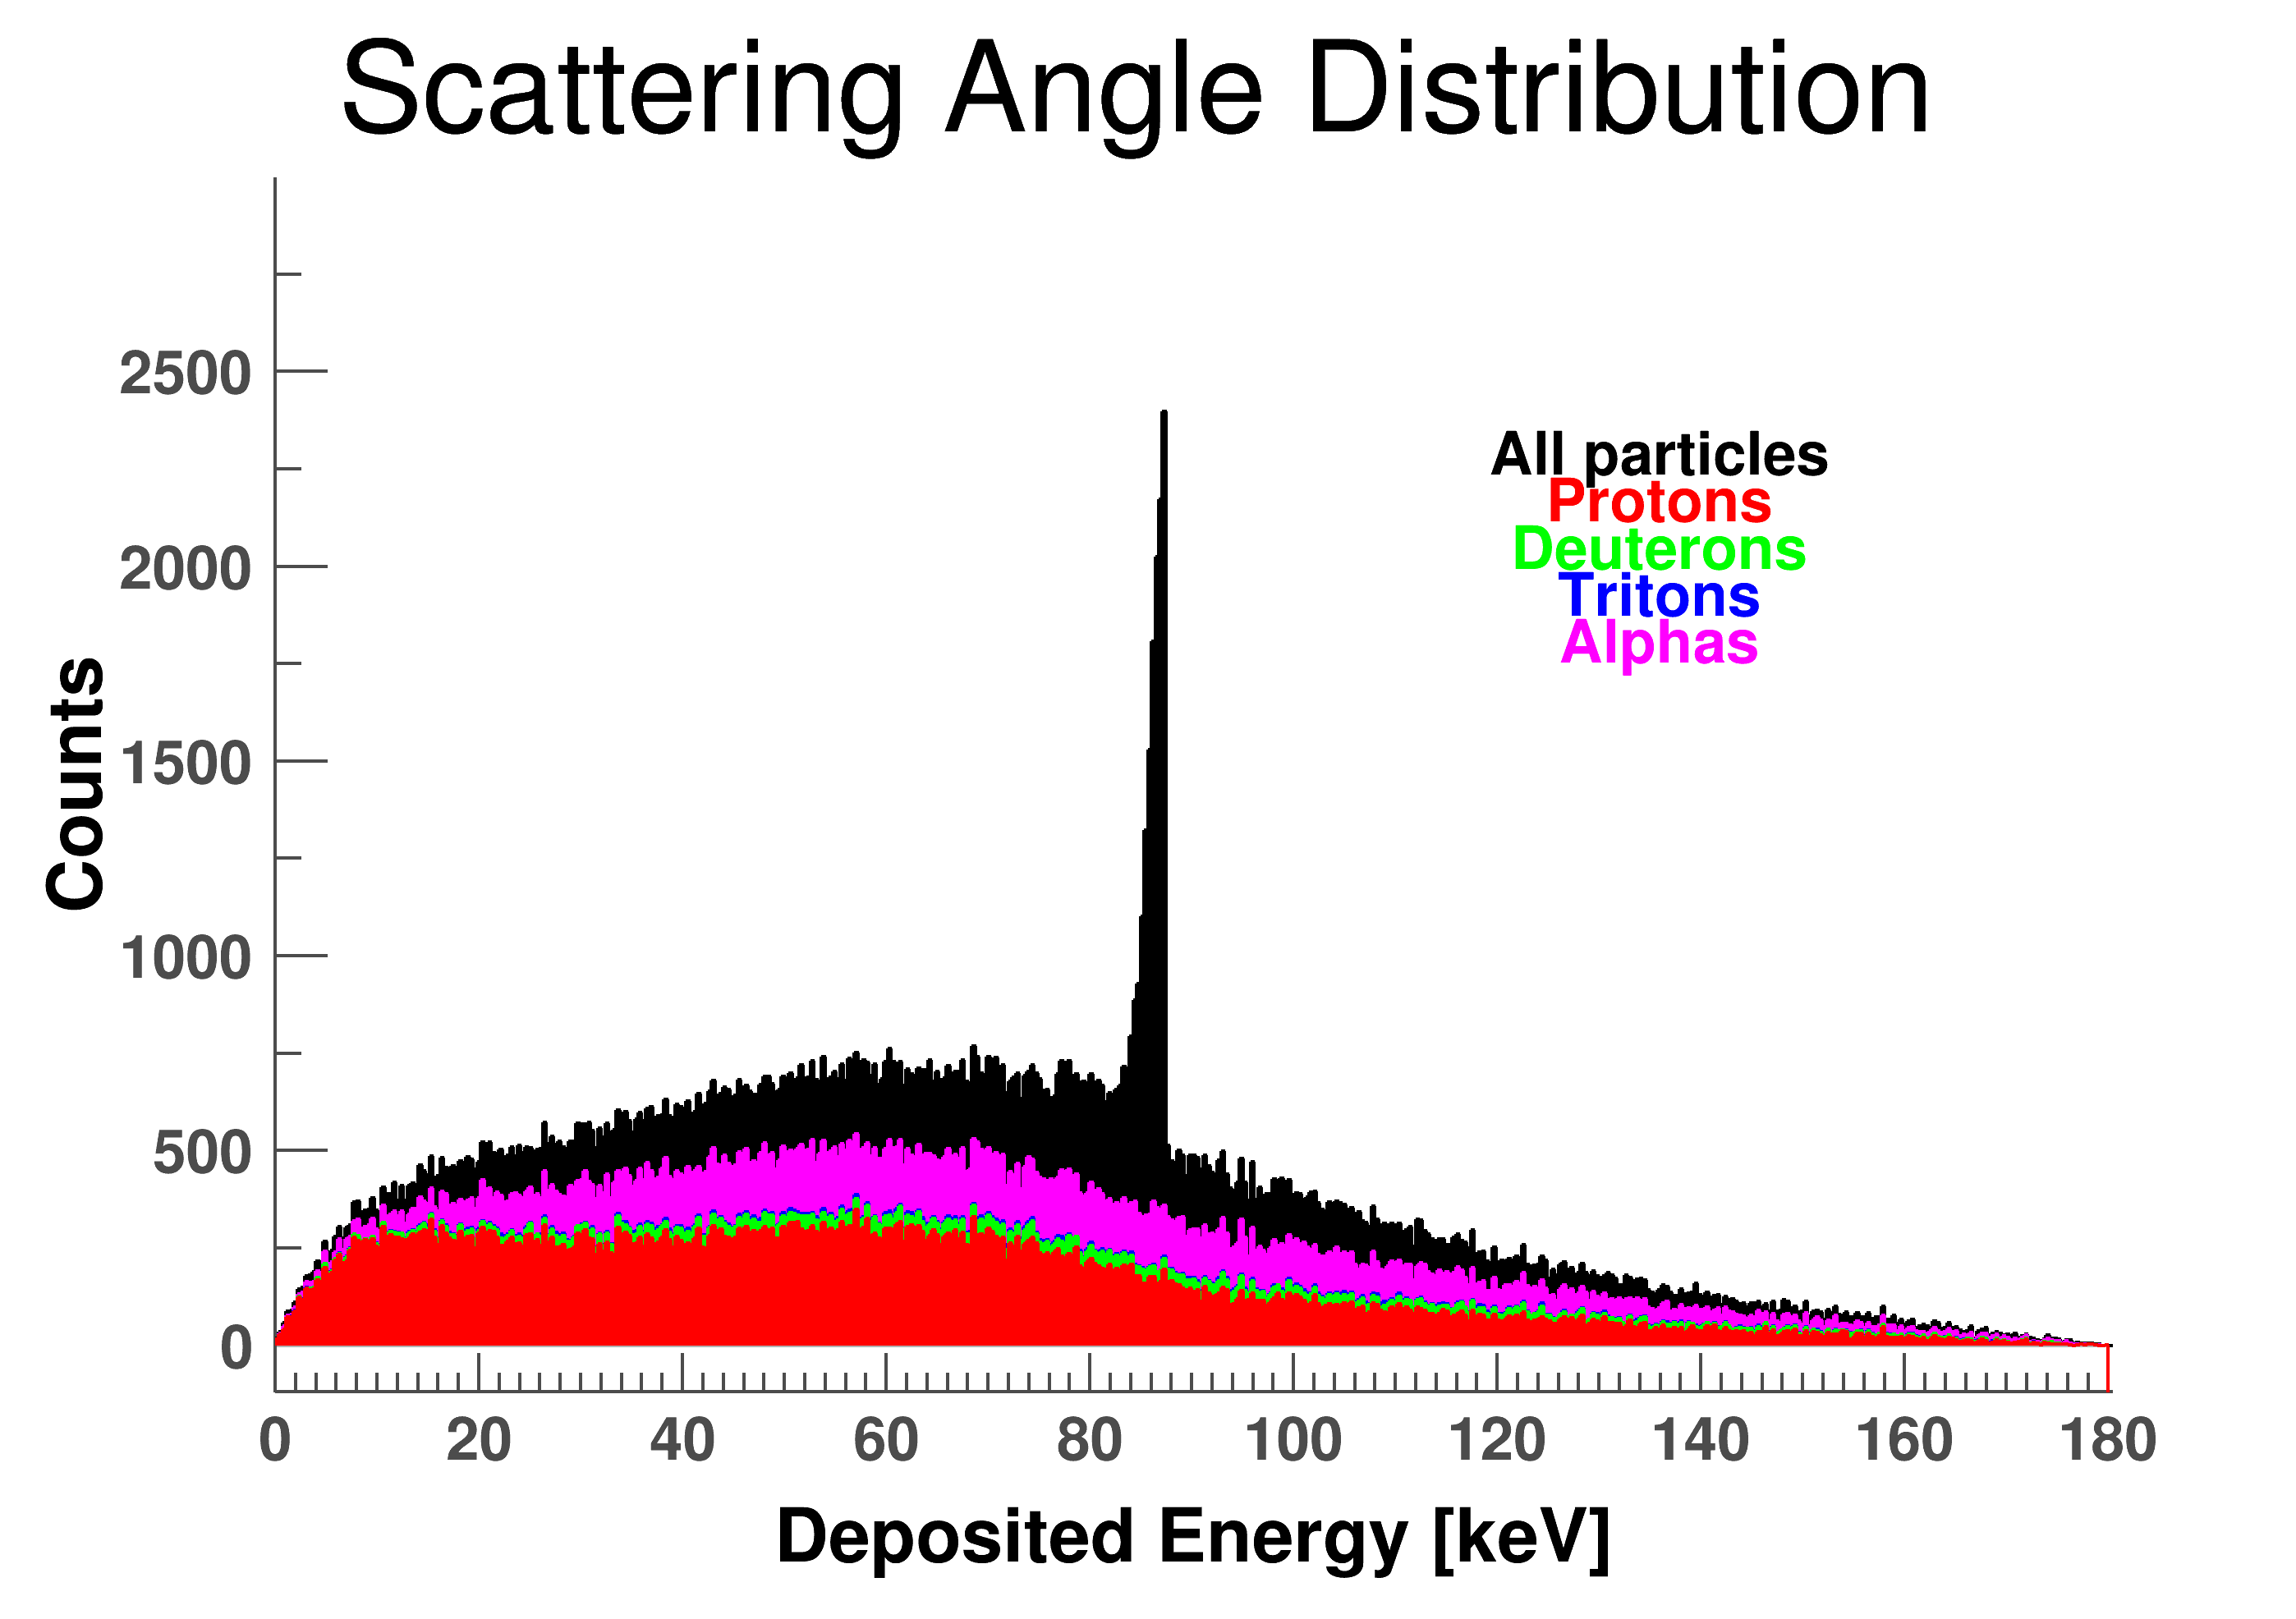
\includegraphics[width=\textwidth]{./A6_QBBC_Scat.png}
    \end{subfigure}
    
    \vspace{1mm}
    
    \begin{subfigure}[htbp]{0.42\textwidth}
        \subcaption{\textbf{Physics List ${=}$ SchieldingM}}
        \label{fig:A7}
        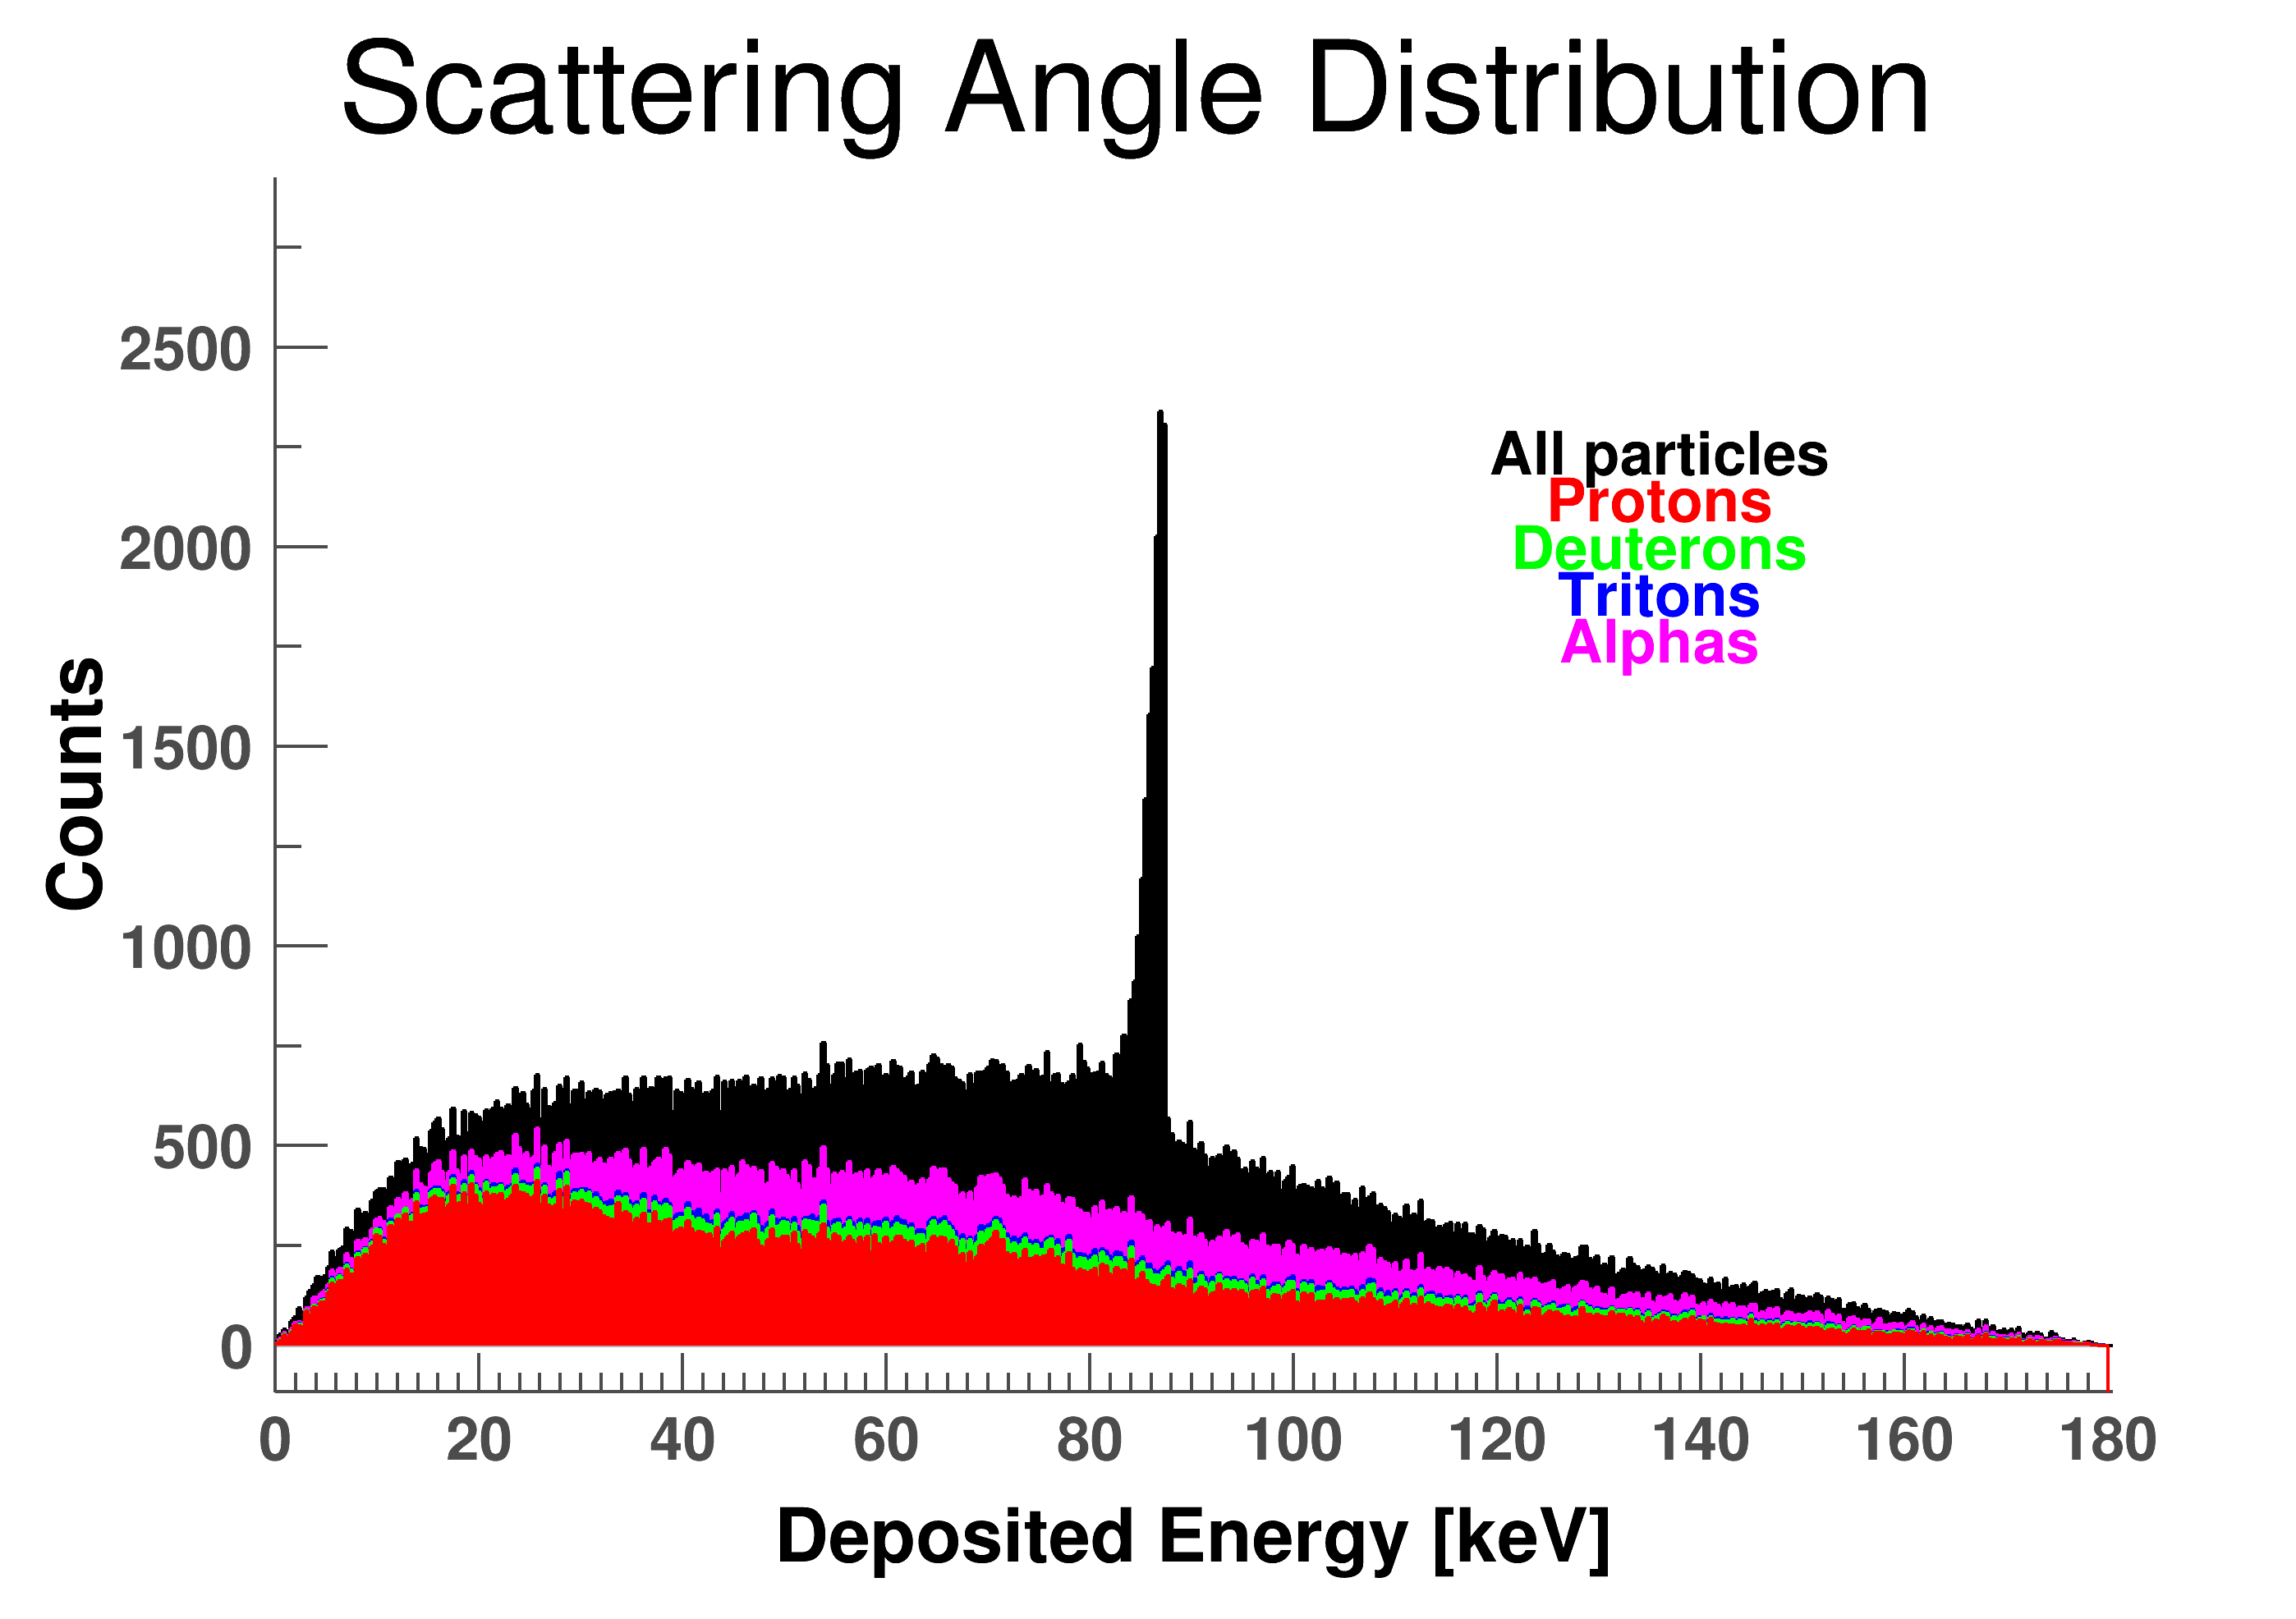
\includegraphics[width=\textwidth]{./A7_ShieldingM_Scat.png}
    \end{subfigure}
    \caption{Scattering angles for different physics lists}
    \label{fig:Alpha}
\end{figure}

%%%%%%%%%%%%%%%%%%%%%%%%%%%%%%%%%%%%%%%%%%%%%%%%%%%%%%%%%%%%%%%%%%%%%%%%%

\begin{figure}[htbp]
    \centering
    \begin{subfigure}[htbp]{0.42\textwidth}
        \subcaption{\textbf{Physics List ${=}$ FTFP-INCLXX-HP}}
        \label{fig:E1}
        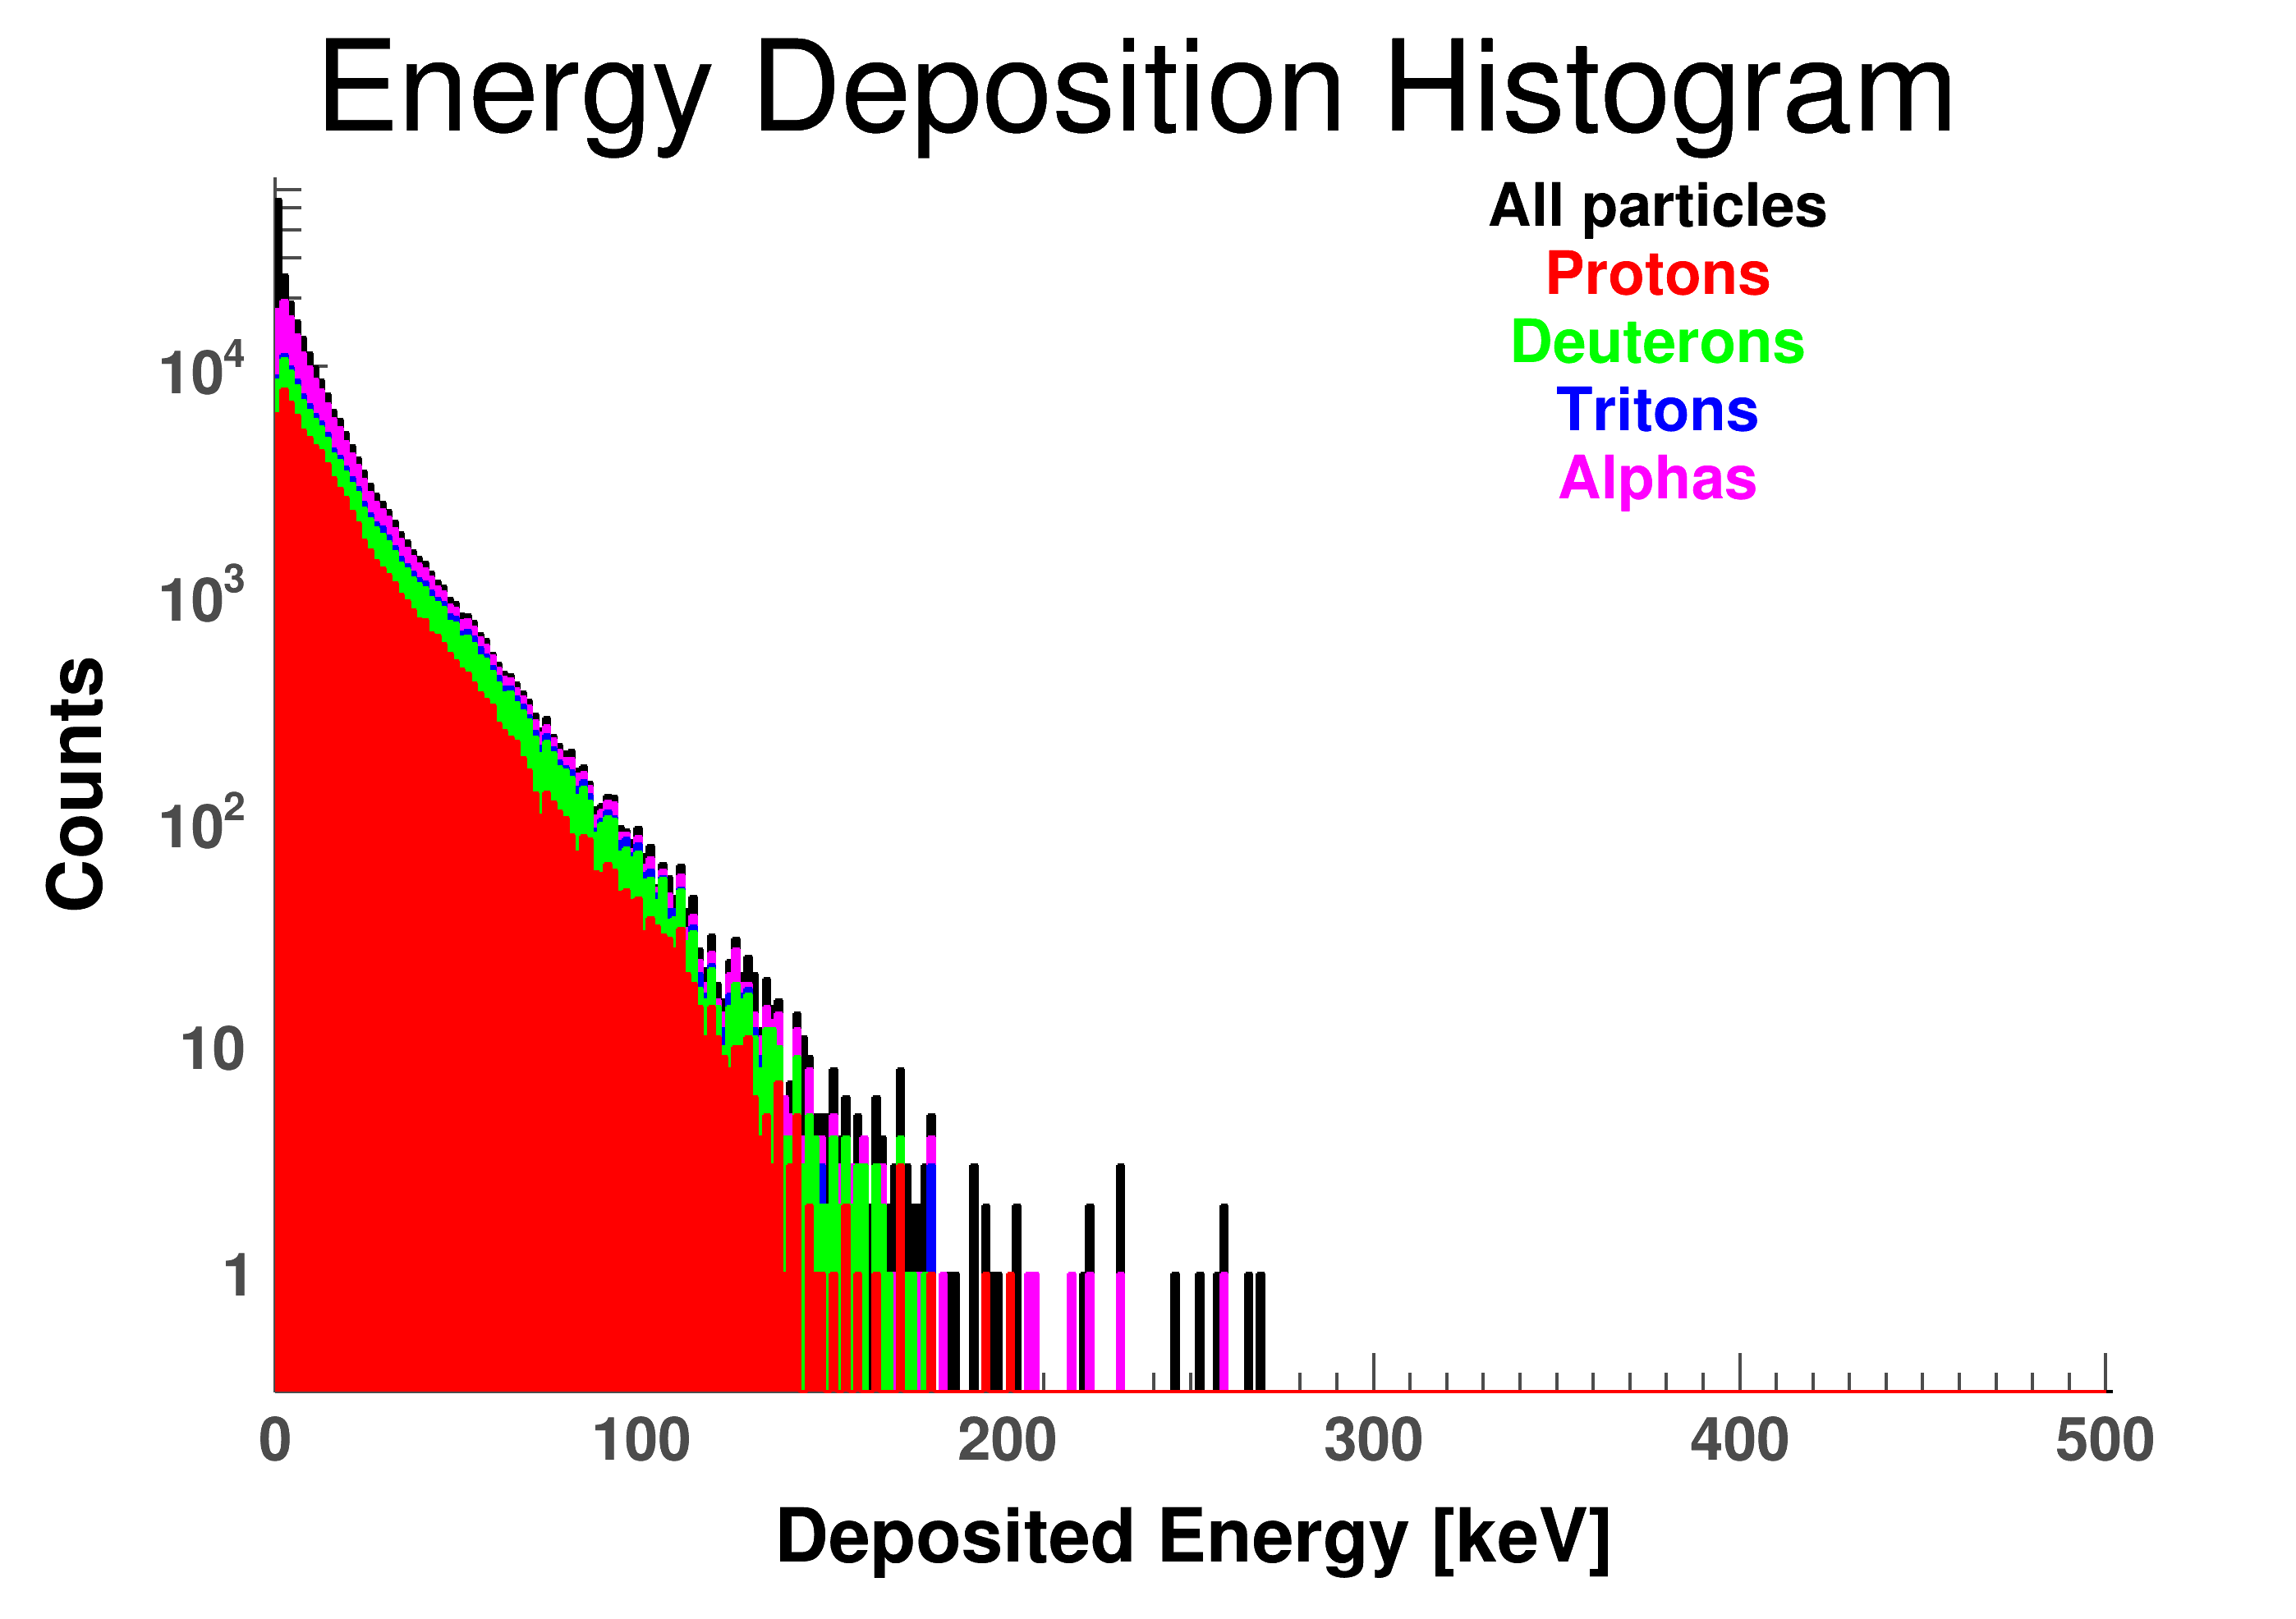
\includegraphics[width=\textwidth]{./E1_FTFP_INCLXX_HP_Edep.png}
    \end{subfigure}
    ~ 
    \begin{subfigure}[htbp]{0.42\textwidth}
        \subcaption{\textbf{Physics List ${=}$ QGSP-INCLXX}}
        \label{fig:E2}
        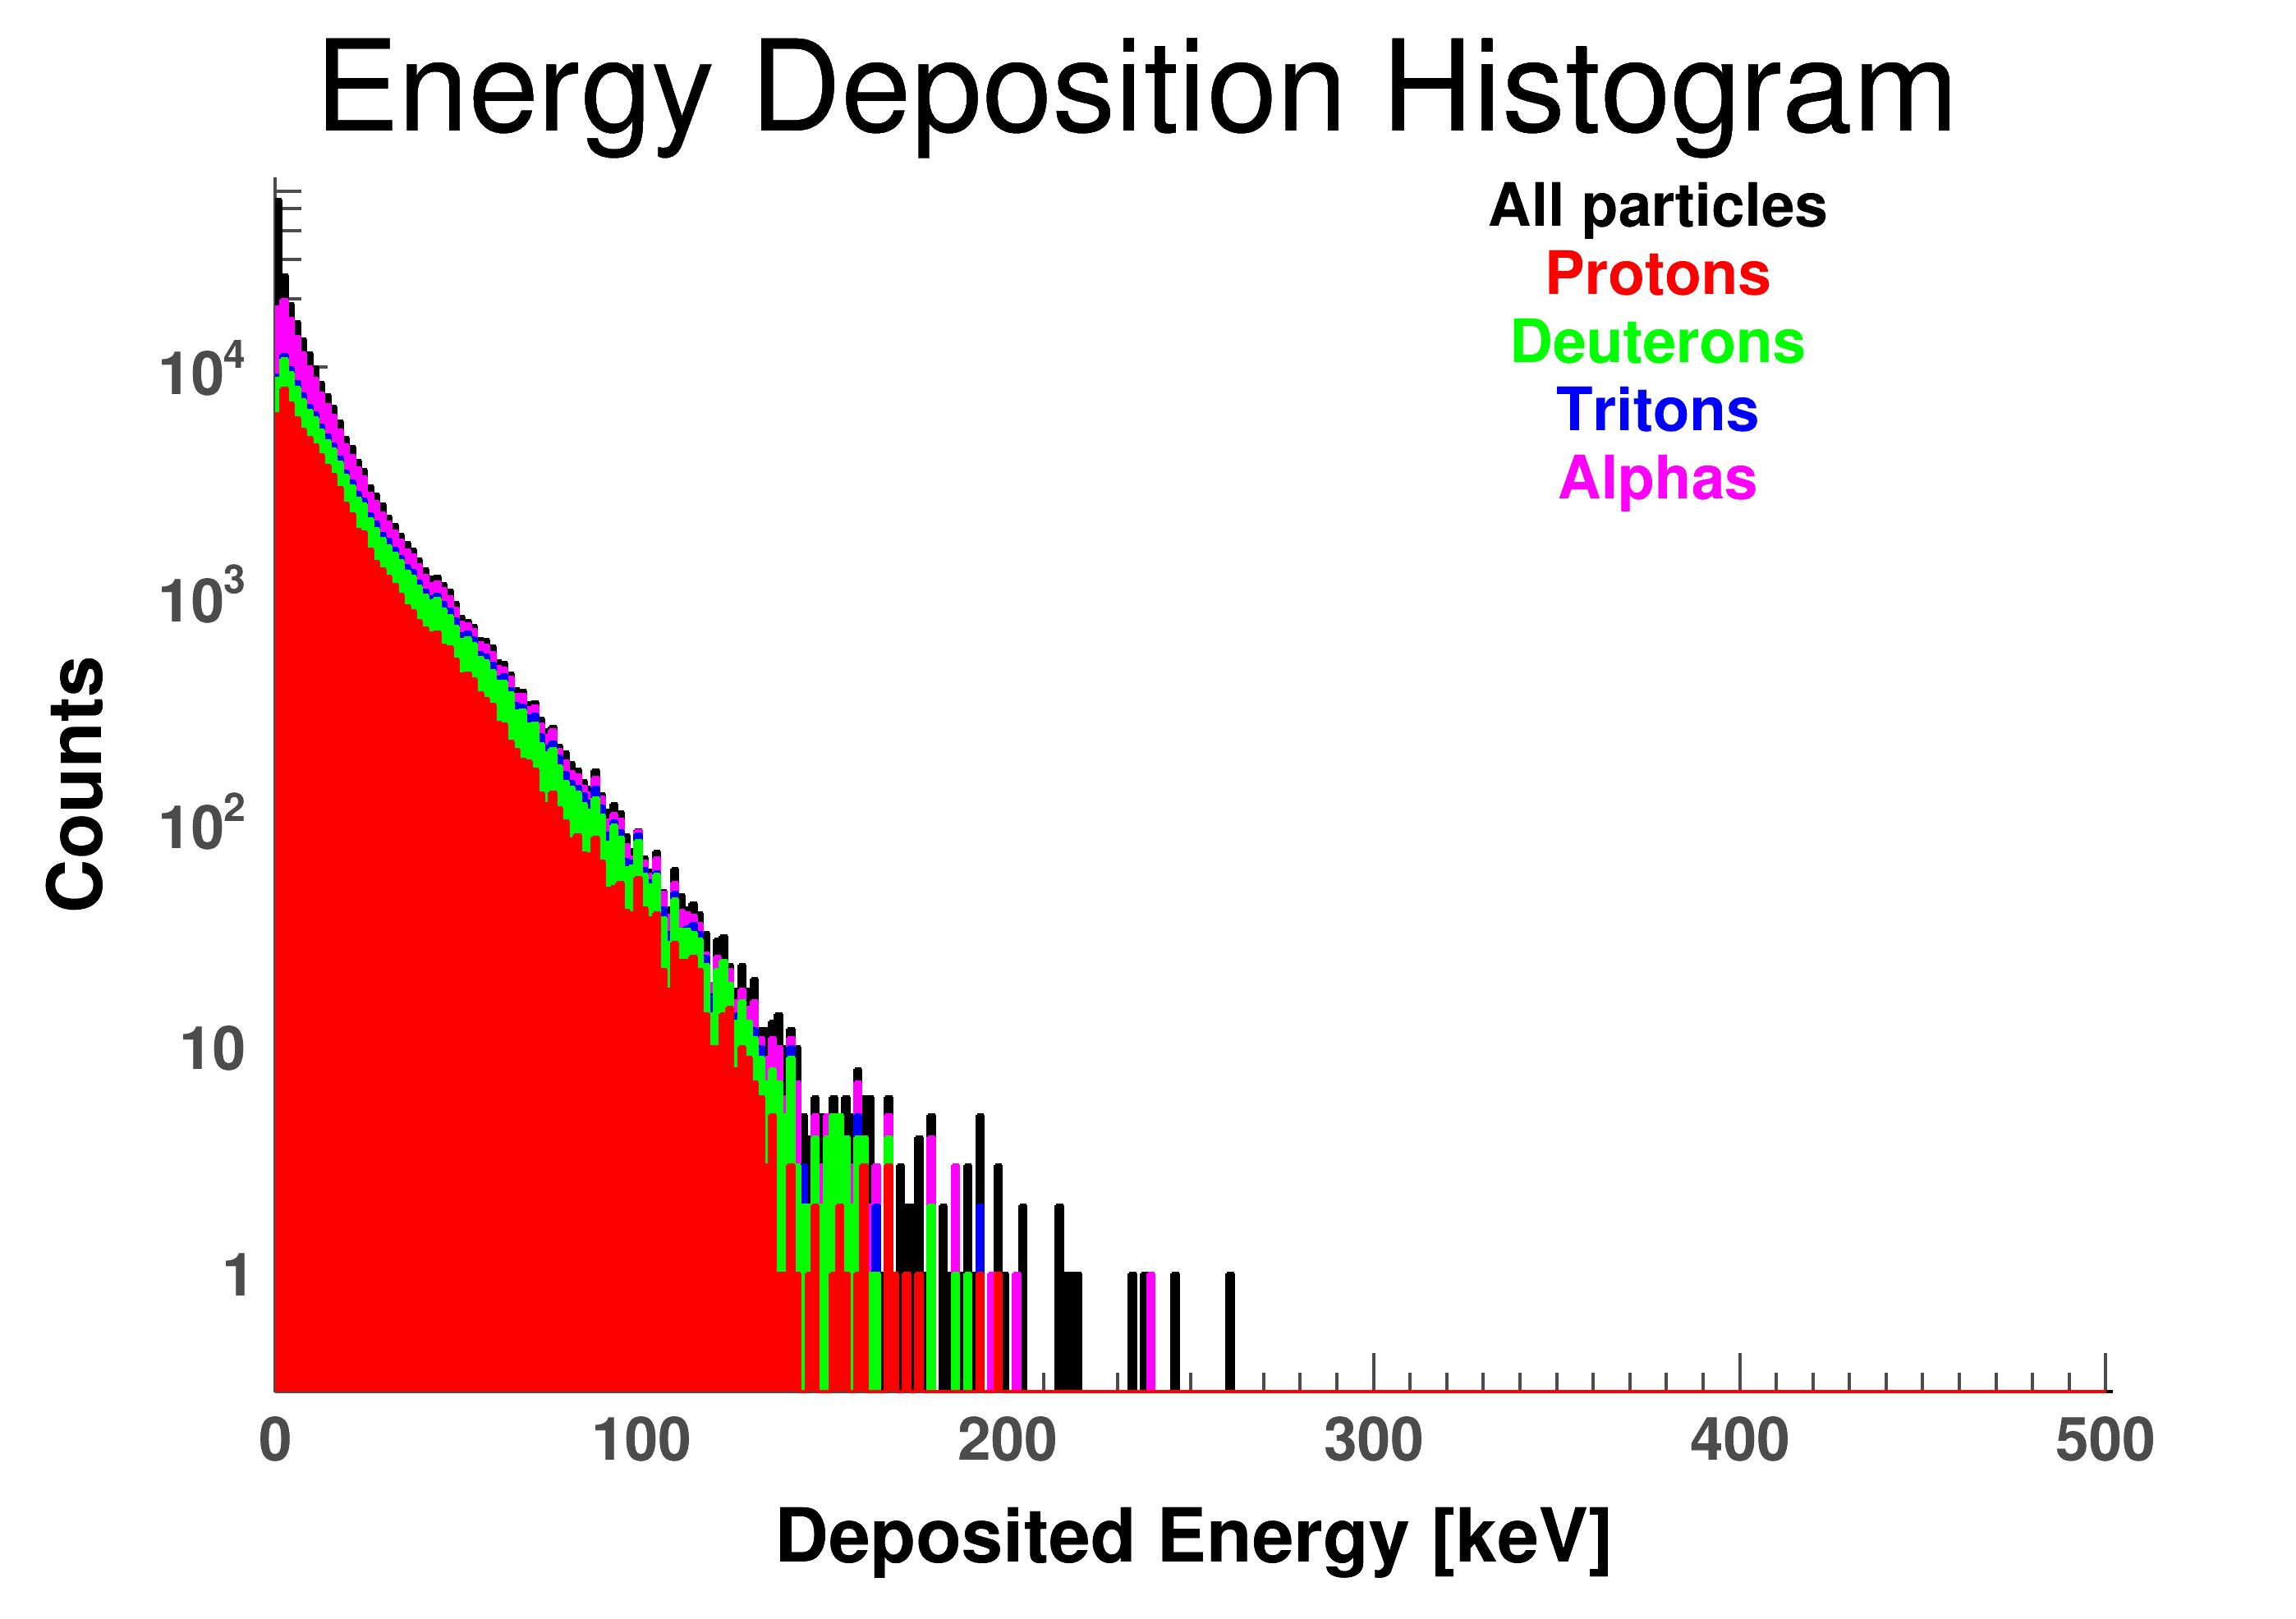
\includegraphics[width=\textwidth]{./E2_QGSP_INCLXX_Edep.png}
    \end{subfigure}
    
    \vspace{1mm}
    
    \begin{subfigure}[htbp]{0.42\textwidth}
        \subcaption{\textbf{Physics List ${=}$ QGSP-INCLXX-HP}}
        \label{fig:E3}
        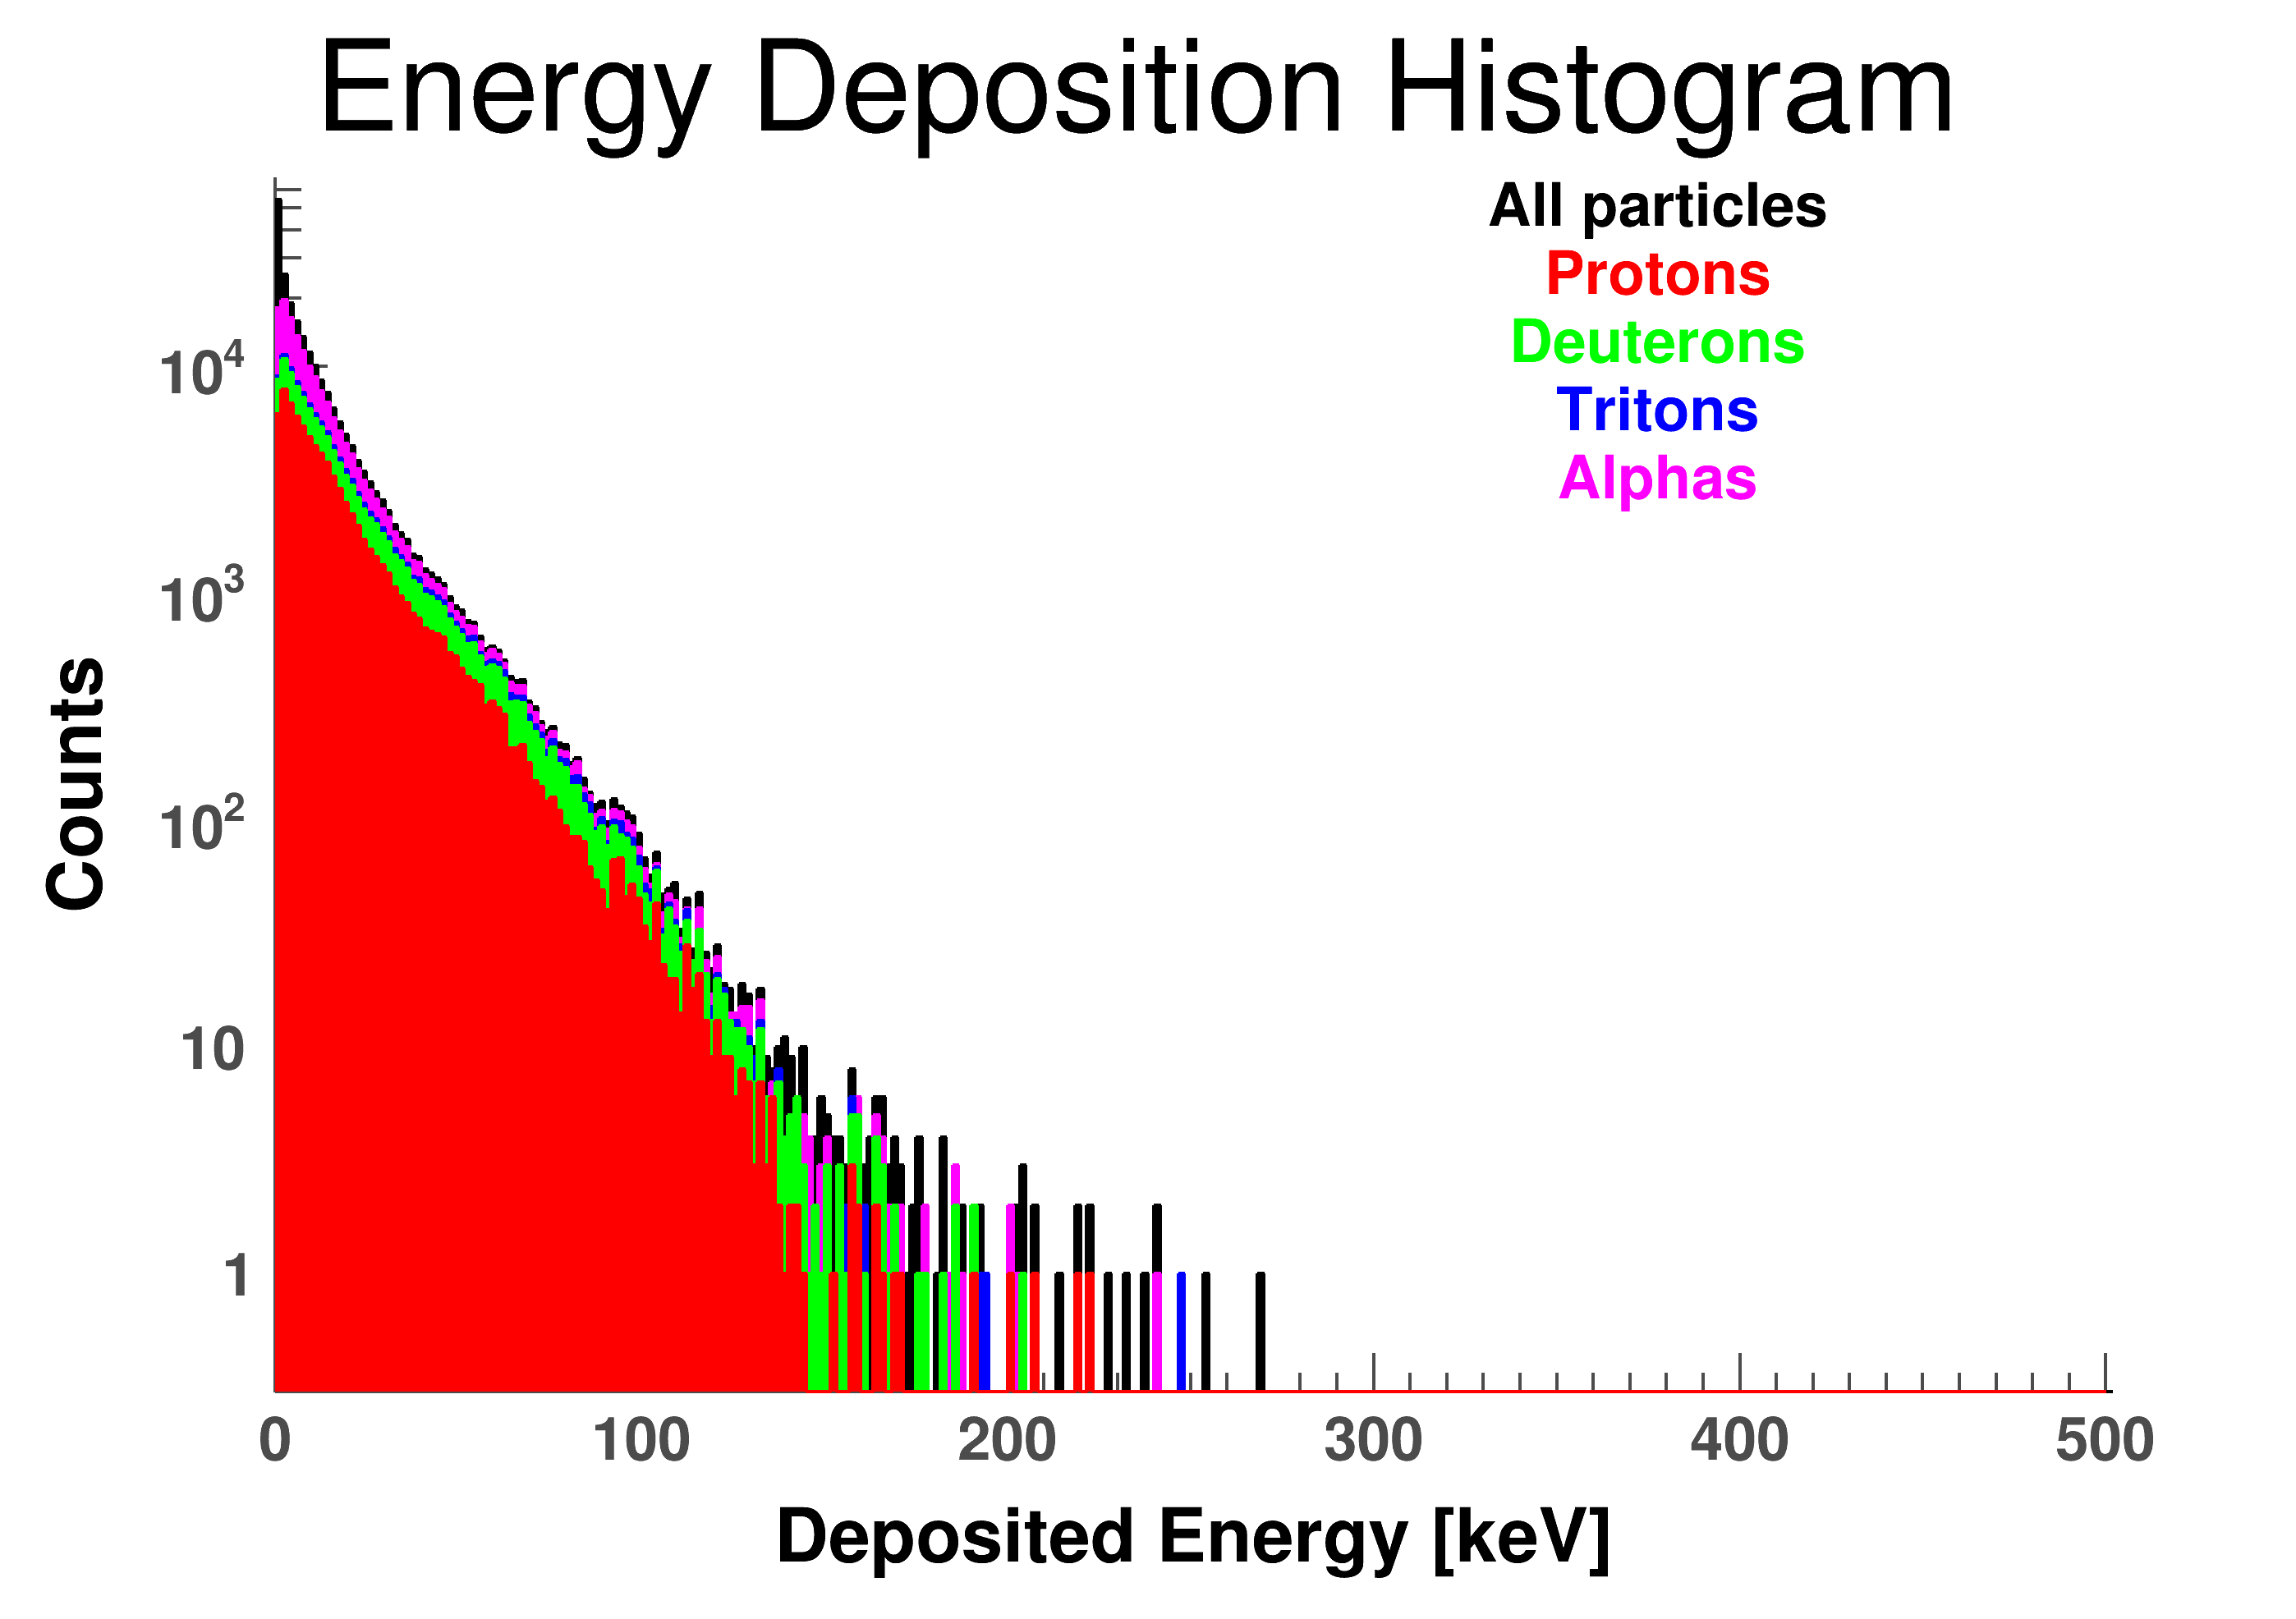
\includegraphics[width=\textwidth]{./E3_QGSP_INCLXX_HP_Edep.png}
    \end{subfigure}
    ~ 
    \begin{subfigure}[htbp]{0.42\textwidth}
        \subcaption{\textbf{Physics List ${=}$ QGSP-BERT-HP}}
        \label{fig:E4}
        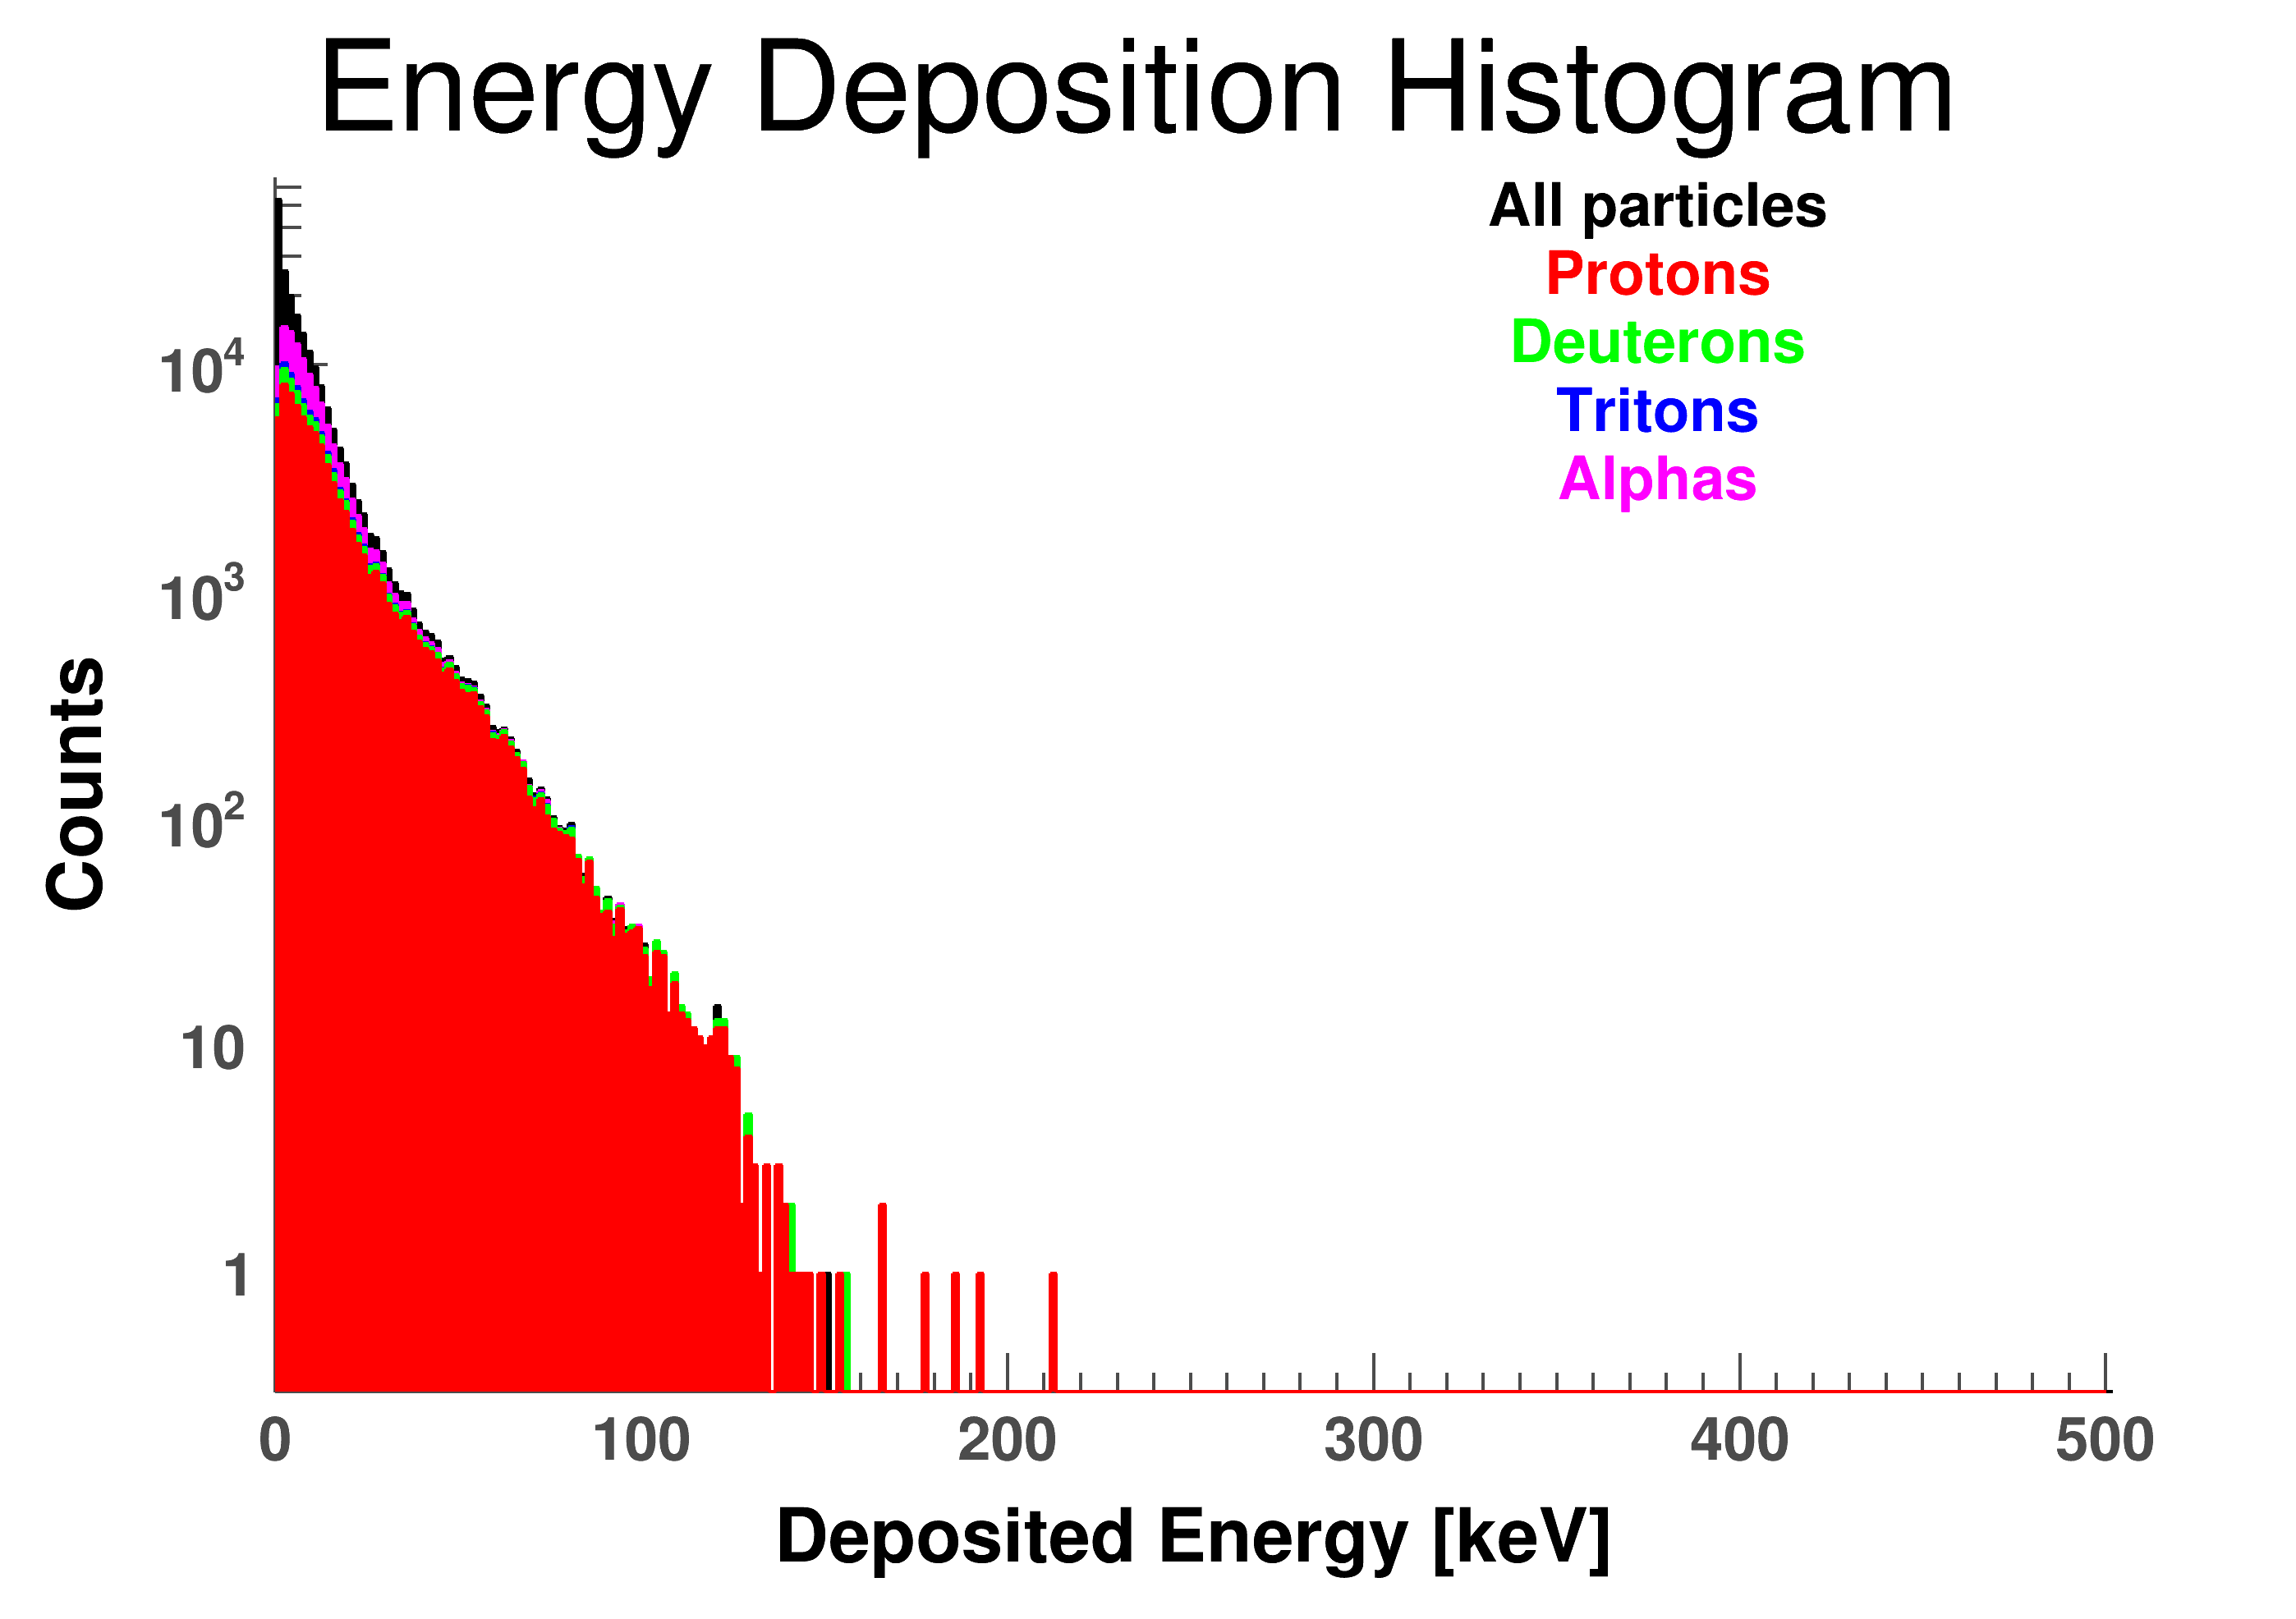
\includegraphics[width=\textwidth]{./E4_QGSP_BERT_HP_Edep.png}
    \end{subfigure}
    
    \vspace{1mm}
    
    \begin{subfigure}[htbp]{0.42\textwidth}
        \subcaption{\textbf{Physics List ${=}$ QGSP-BIC-HP}}
        \label{fig:E5}
        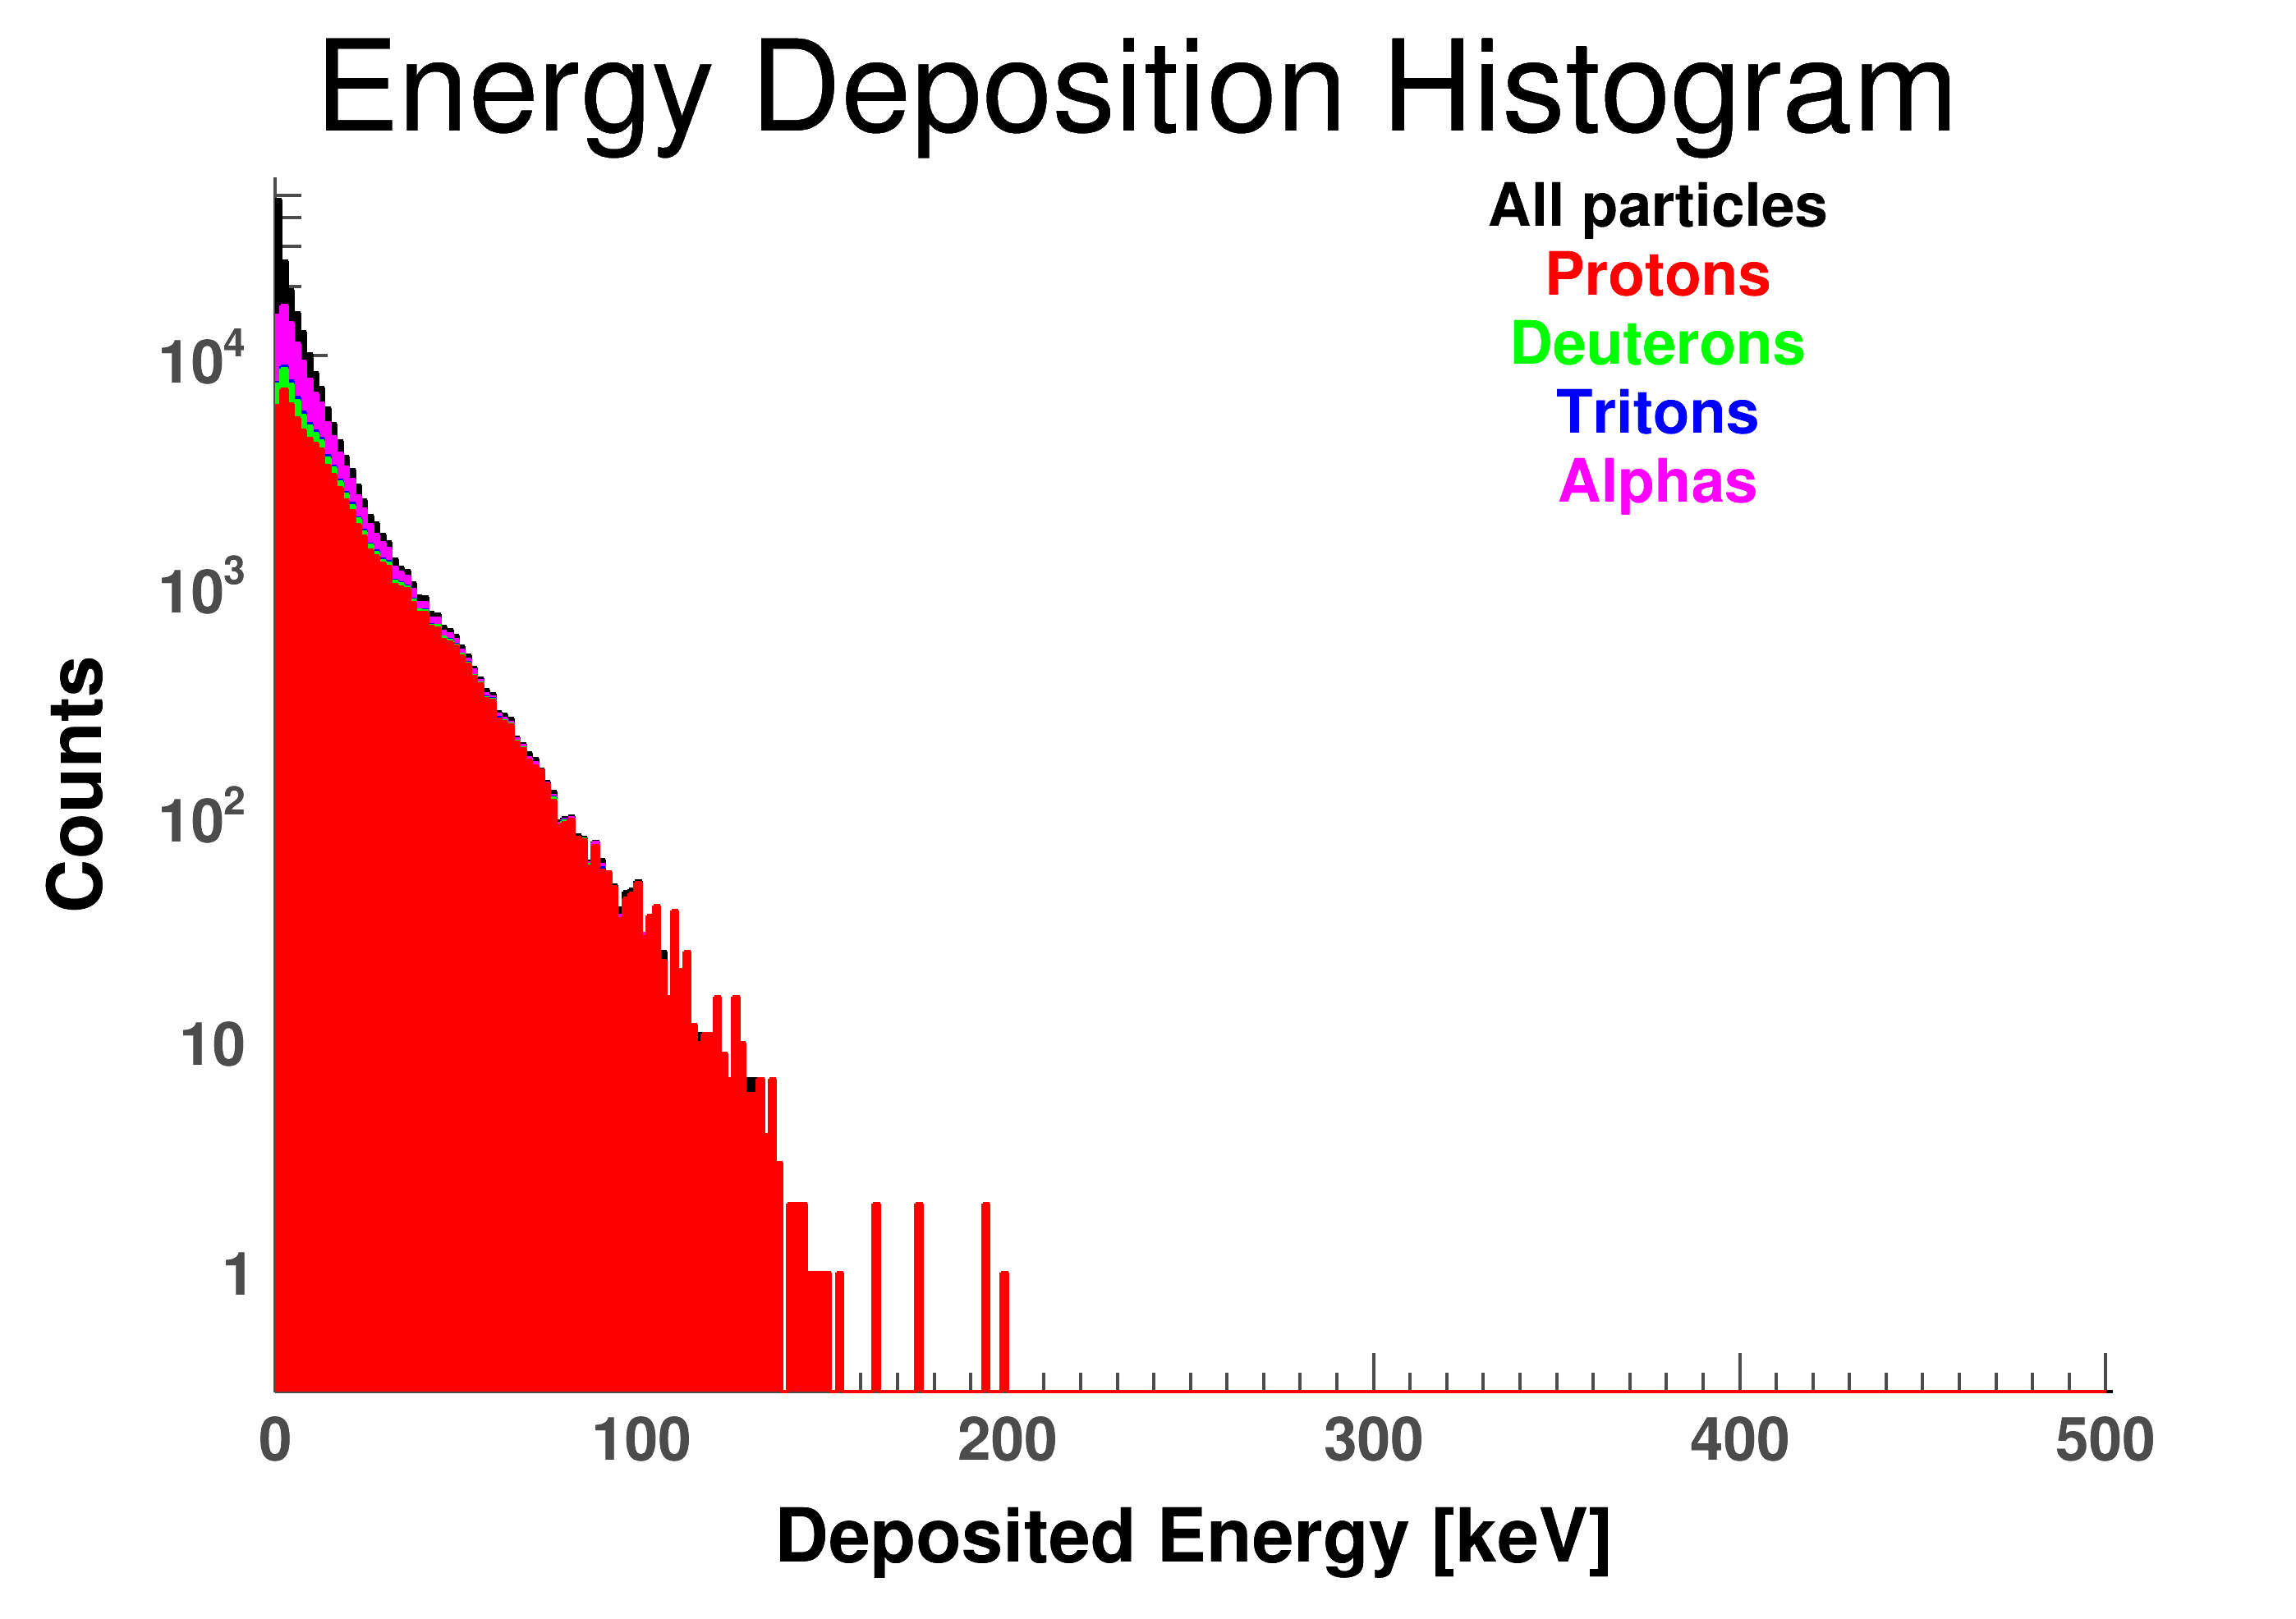
\includegraphics[width=\textwidth]{./E5_QGSP_BIC_HP_Edep.png}
    \end{subfigure}
    ~ 
    \begin{subfigure}[htbp]{0.42\textwidth} 
        \subcaption{\textbf{Physics List ${=}$ QBBC}}
        \label{fig:E6}
        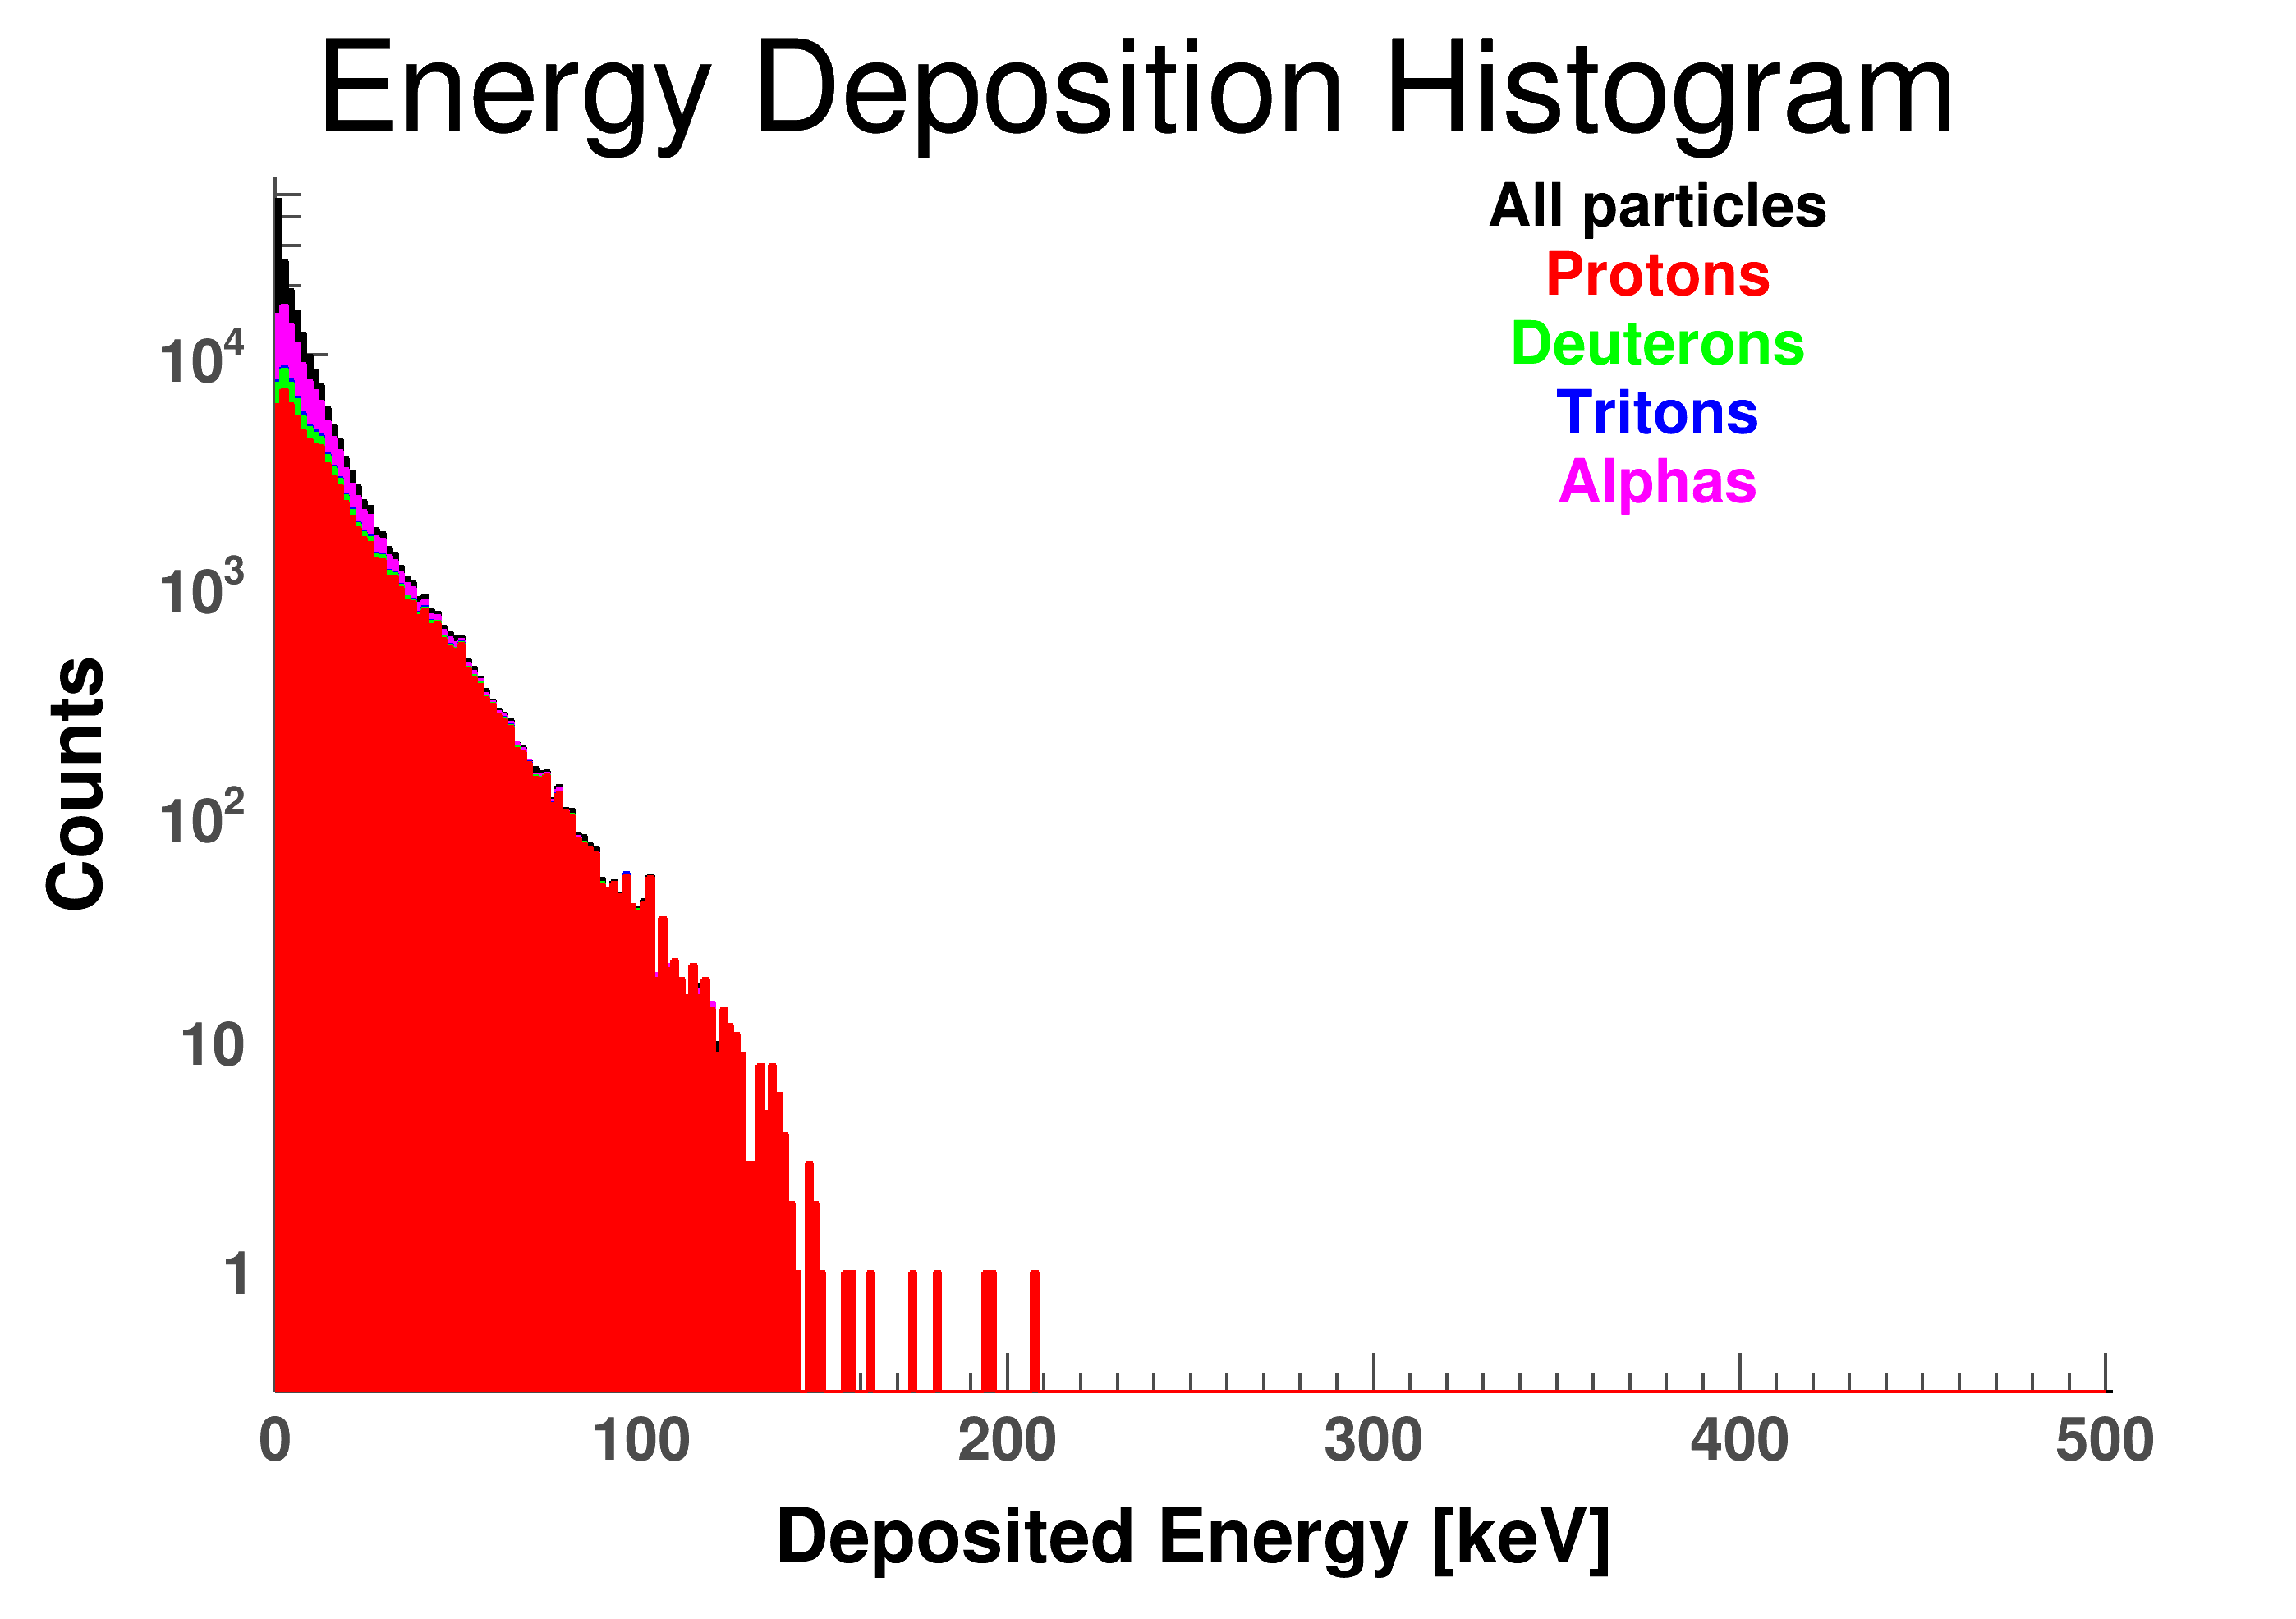
\includegraphics[width=\textwidth]{./E6_QBBC_Edep.png}
    \end{subfigure}
    
    \vspace{1mm}
    
    \begin{subfigure}[htbp]{0.42\textwidth}
        \subcaption{\textbf{Physics List ${=}$ SchieldingM}}
        \label{fig:E7}
        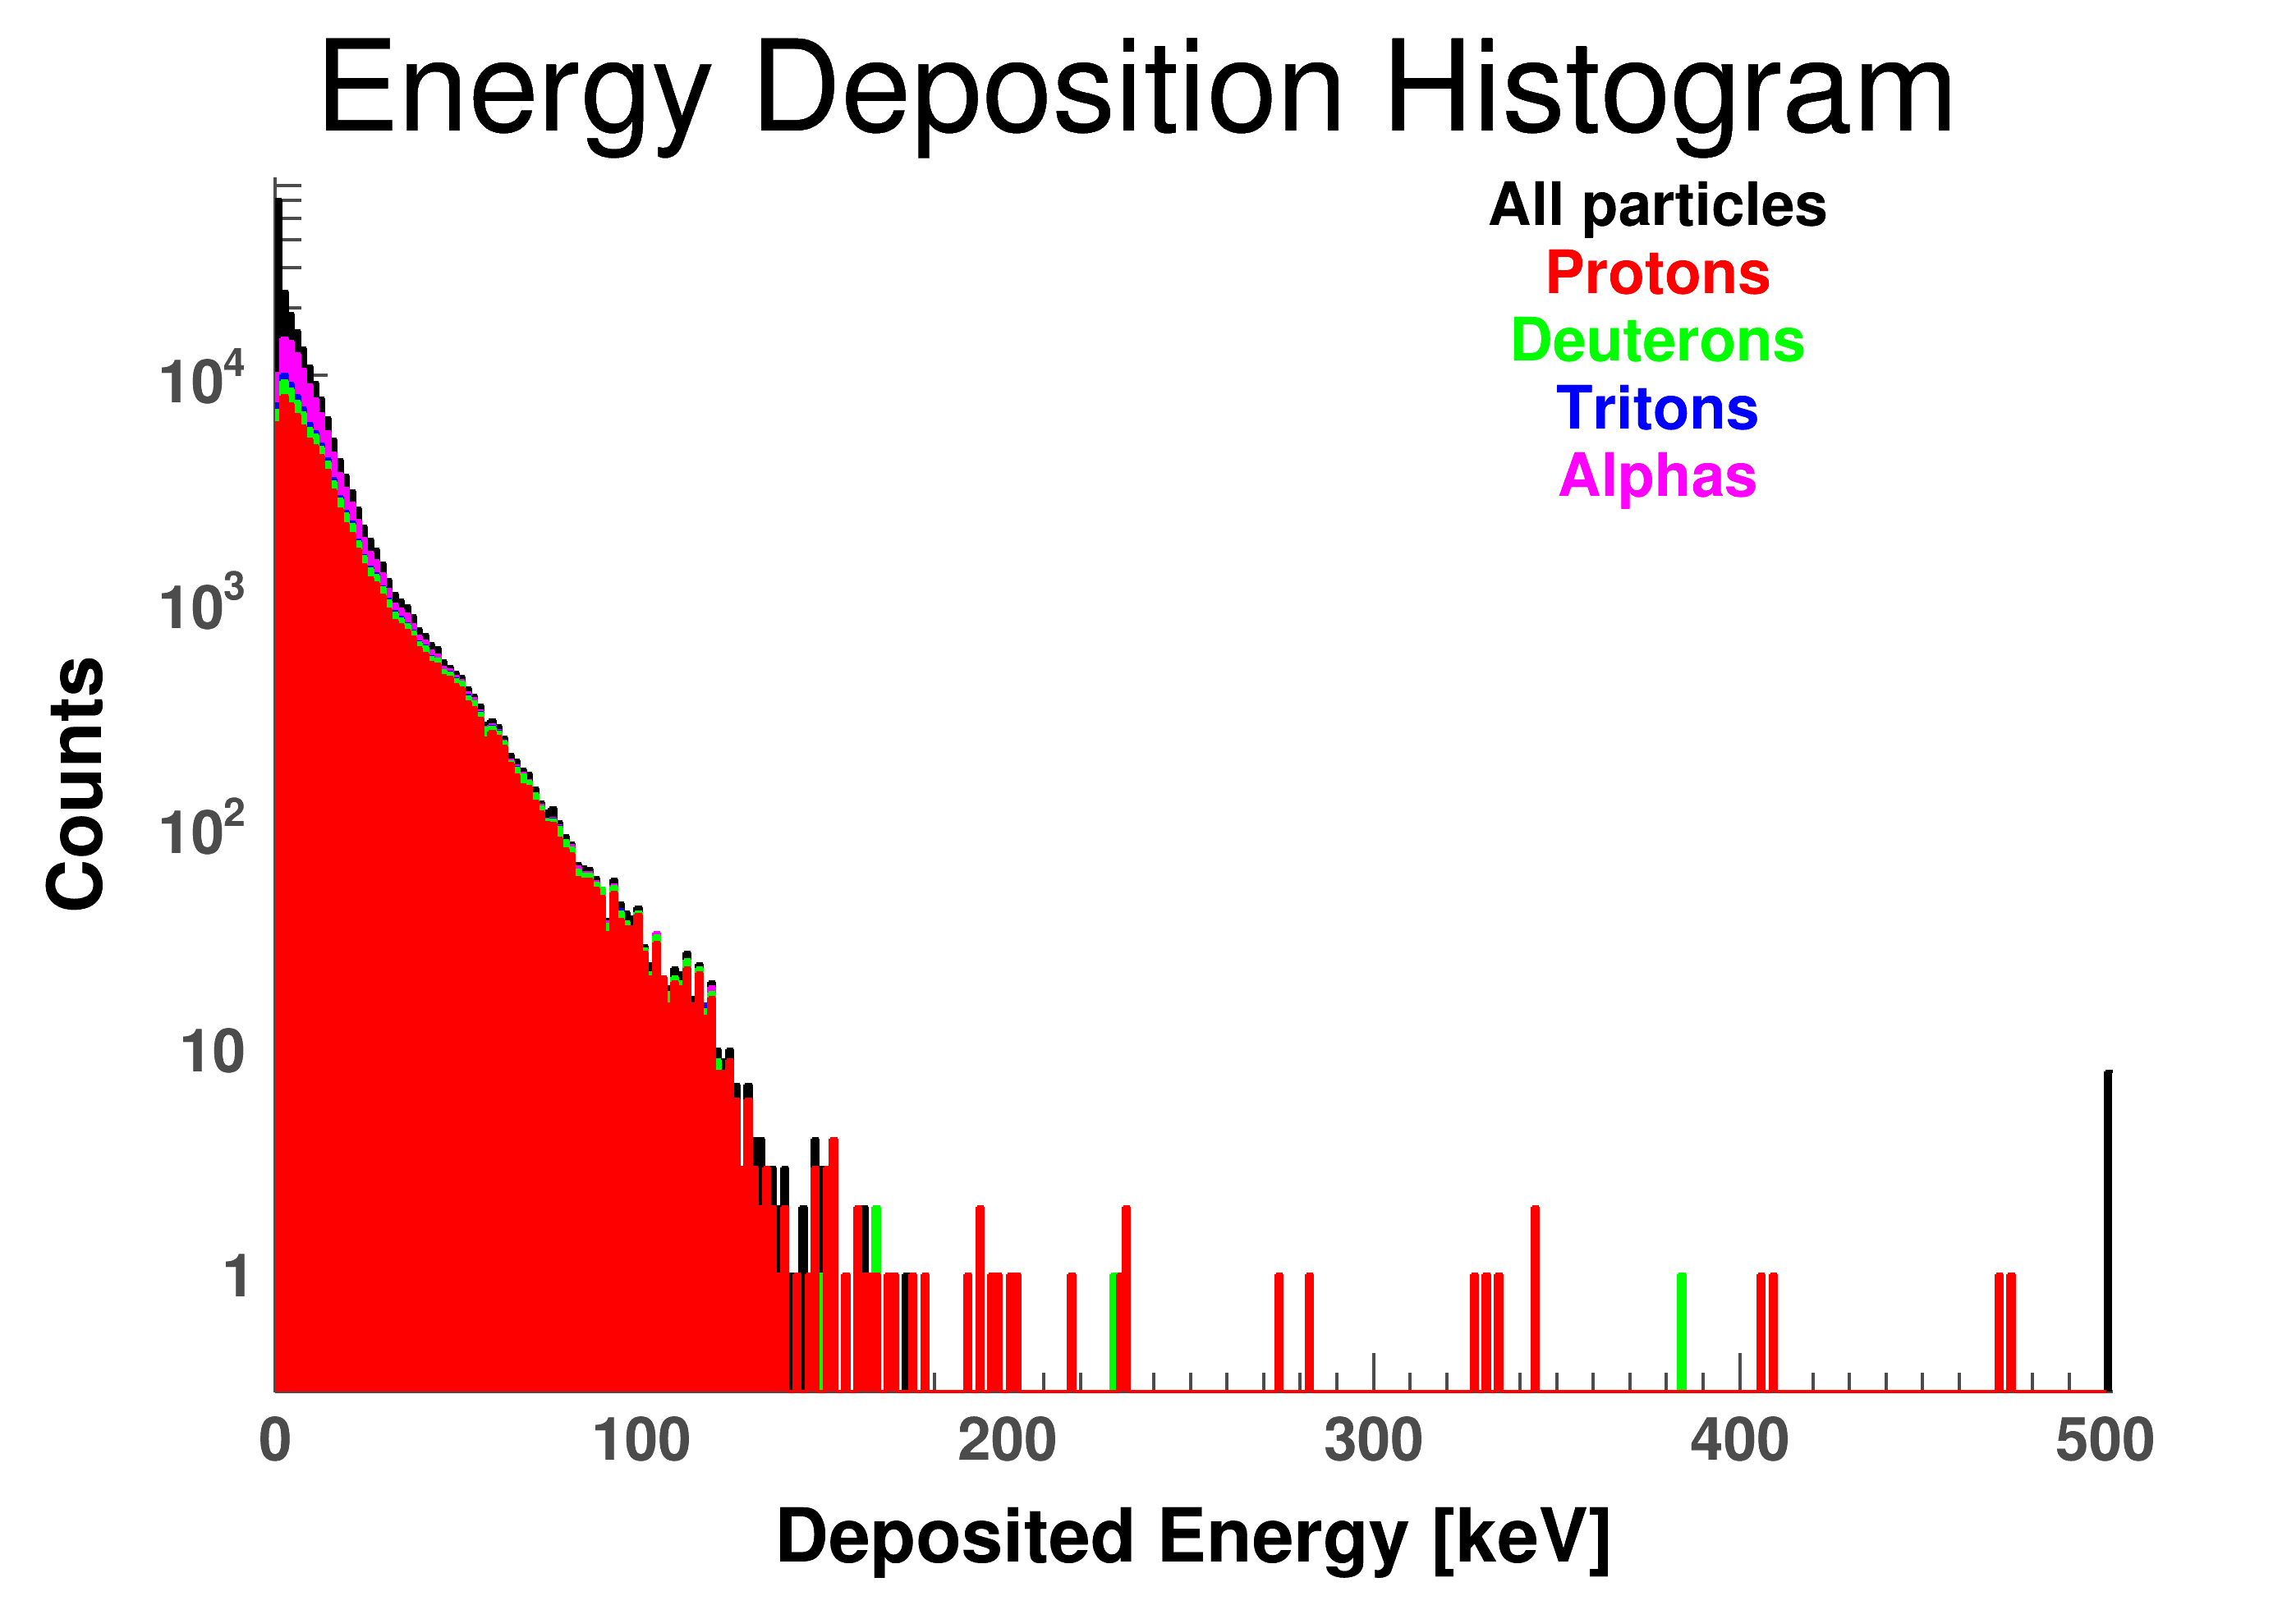
\includegraphics[width=\textwidth]{./E7_ShieldingM_Edep.png}
    \end{subfigure}
    \caption{Energy depositions for different physics lists} 
    \label{fig:Edep}
\end{figure}

%%%%%%%%%%%%%%%%%%%%%%%%%%%%%%%%%%%%%%%%%%%%%%%%%%%%%%%%%%%%%%%

\begin{figure}
\centering
  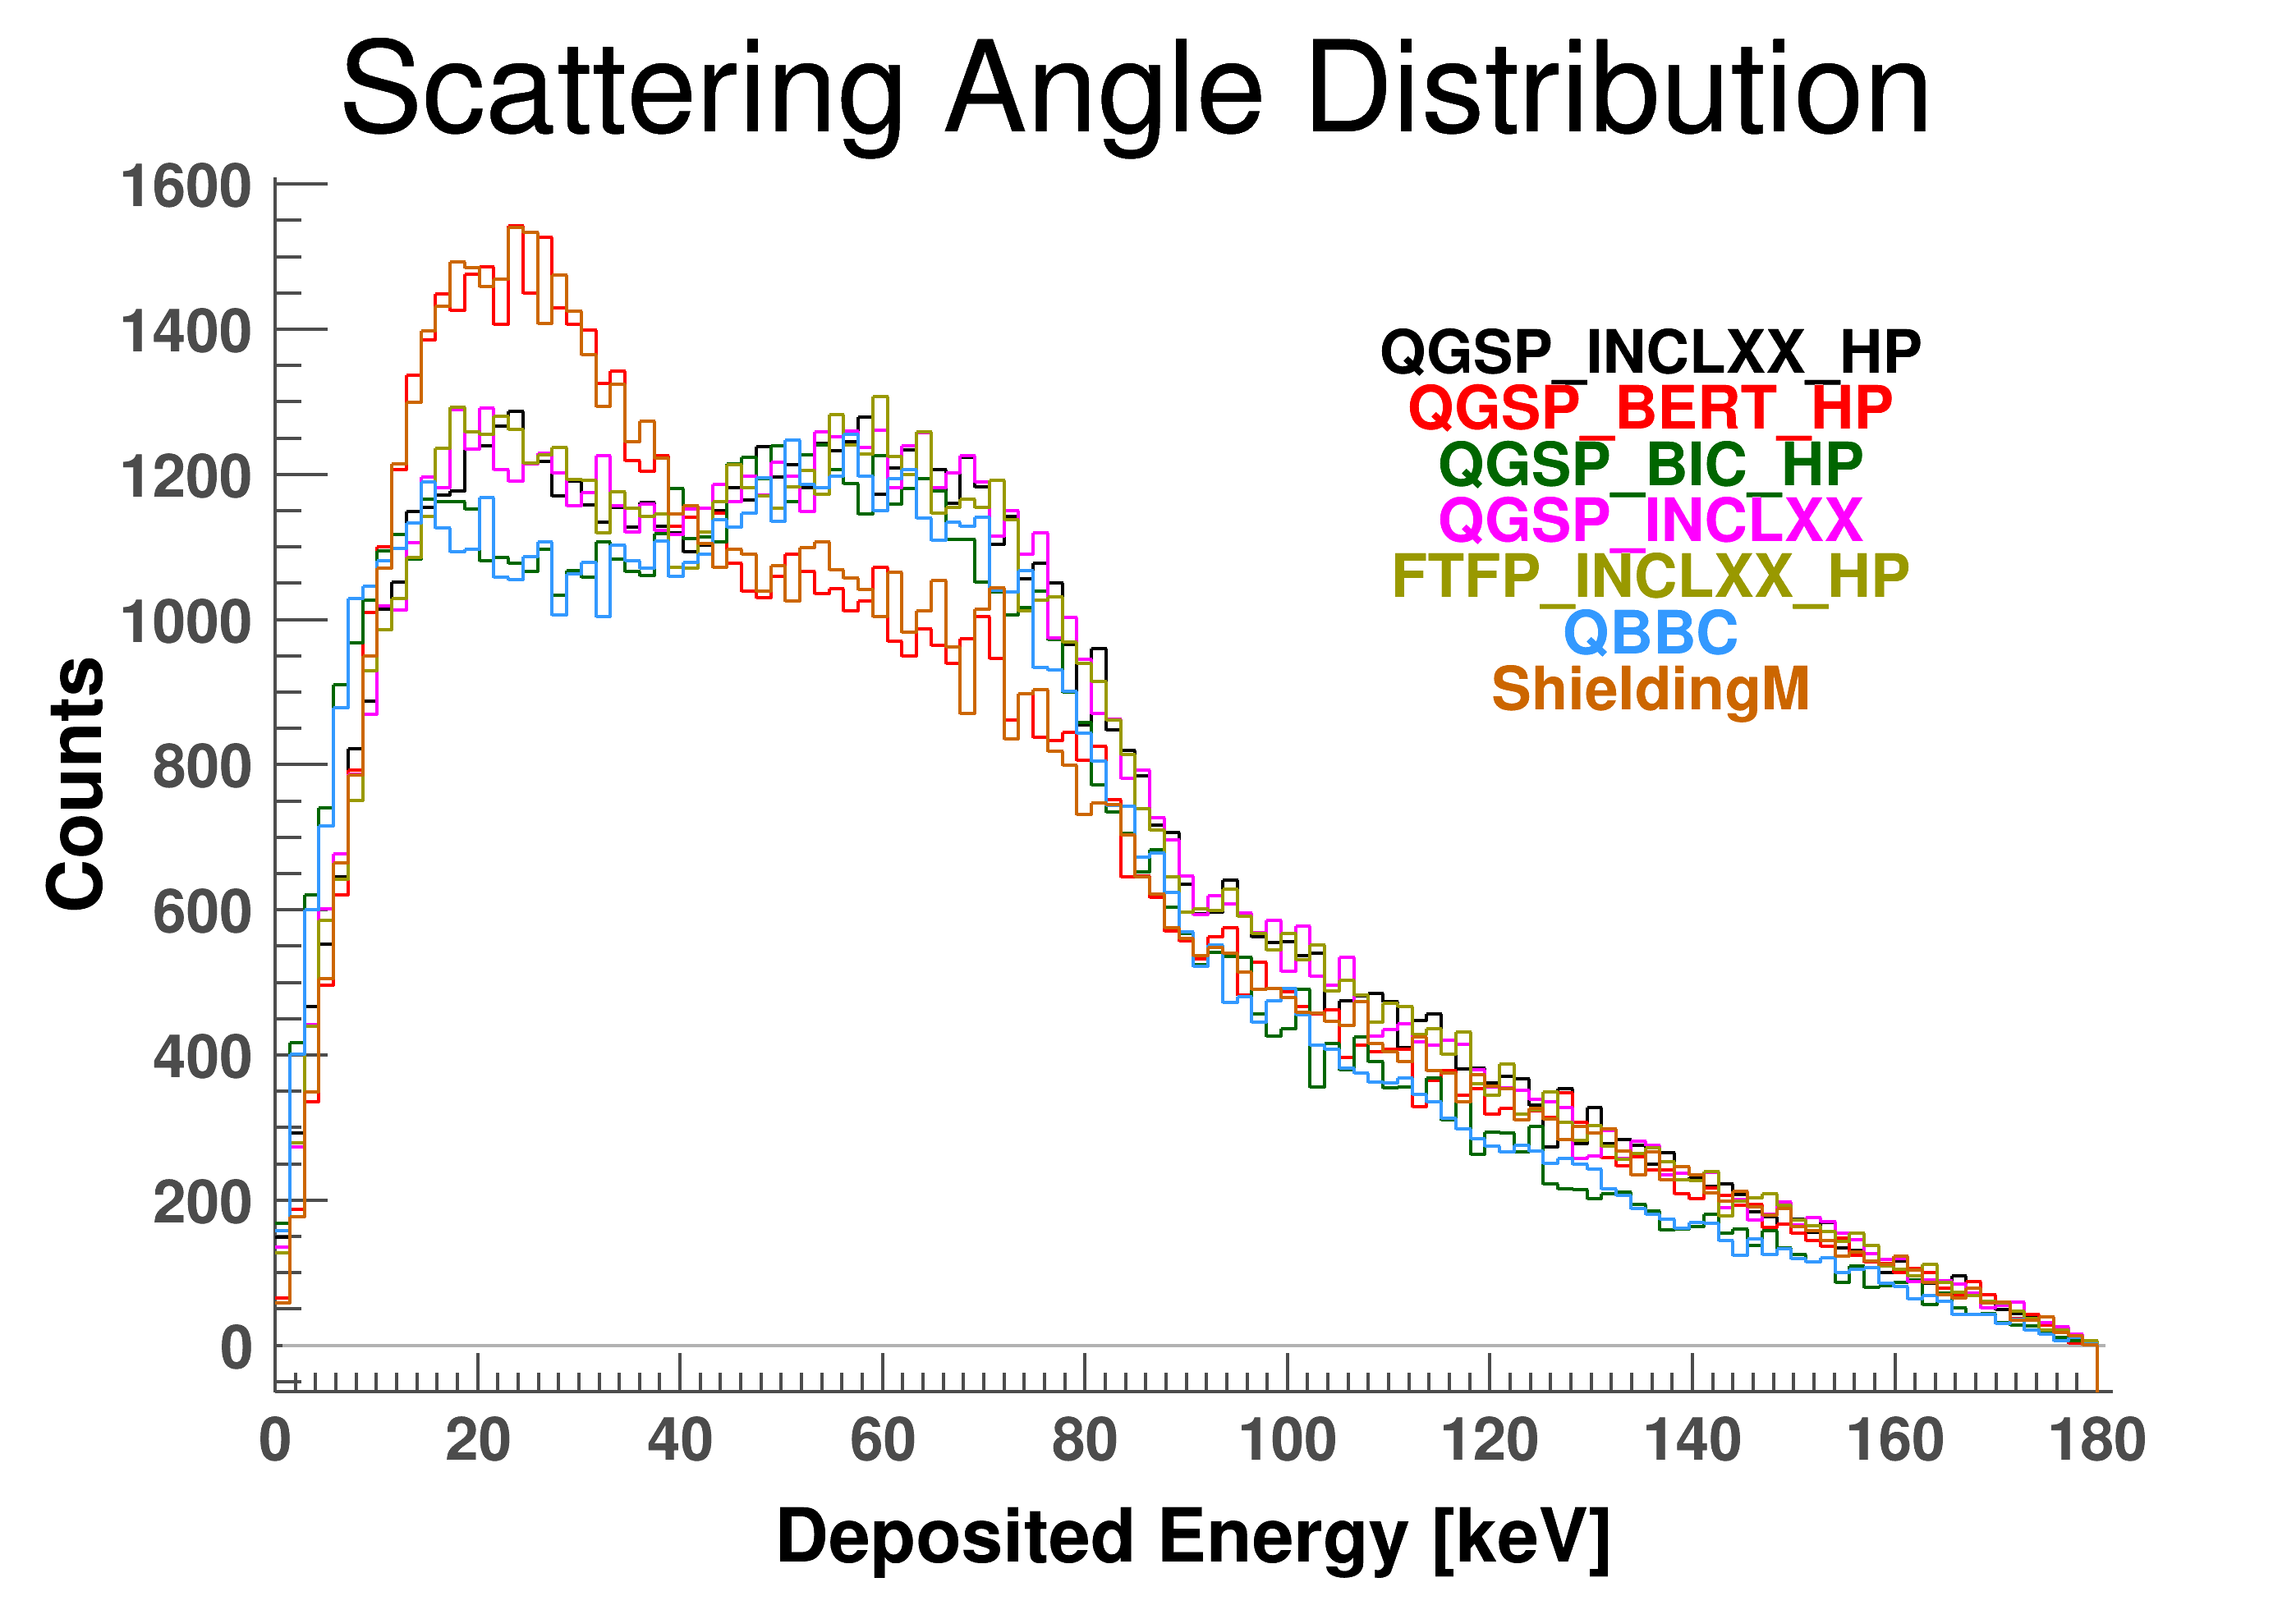
\includegraphics[width=1.00\textwidth]{./ProtonScattering.png}
  \caption{Proton scattering angles for different physics lists}  
  \label{fig:ProtonAlpha}
\end{figure}

%%%%%%%%%%%%%%%%%%%%%%%%%%%%%%%%%%%%%%%%%%%%%%%%%%%%%%%%%%%%%%%

\FloatBarrier
\section{Tranditional methods for different numbers of double-planes}
\label{sec:tradmed_dp} 

\begin{table}[htbp]
\centering
\caption{Traditional method results TRAINING/VALIDATION for \textrm{4dp} at ${600 \MeV}$ neutrons.}
\label{tab:4dp600}
\begin{tabular}{| c | c c c c | c c |}
\hline
Mult. & INCLXX/INCLXX & BERT/INCLXX & INCLXX/BERT & BERT/BERT & Abs. Err. & Rel Err.   \\
\hline
0n    & ${89 \%}$     & ${89 \%}$   & ${90 \%}$   & ${90 \%}$ & ${1 \%}$  & ${1.1 \%}$ \\
1n    & ${55 \%}$     & ${60 \%}$   & ${56 \%}$   & ${62 \%}$ & ${7 \%}$  & ${13 \%}$  \\
2n    & ${48 \%}$     & ${42 \%}$   & ${48 \%}$   & ${41 \%}$ & ${7 \%}$  & ${17 \%}$  \\
3n    & ${38 \%}$     & ${35 \%}$   & ${36 \%}$   & ${34 \%}$ & ${4 \%}$  & ${12 \%}$  \\
4n    & ${36 \%}$     & ${23 \%}$   & ${33 \%}$   & ${23 \%}$ & ${13 \%}$ & ${57 \%}$  \\
5n    & ${39 \%}$     & ${56 \%}$   & ${35 \%}$   & ${51 \%}$ & ${21 \%}$ & ${60 \%}$  \\
\hline
\end{tabular}
\end{table}

\begin{table}[htbp]
\centering
\caption{Traditional method results TRAINING/VALIDATION for \textrm{12dp} at ${600 \MeV}$ neutrons.}
\label{tab:12dp600}
\begin{tabular}{| c | c c c c | c c |}
\hline
Mult. & INCLXX/INCLXX & BERT/INCLXX & INCLXX/BERT & BERT/BERT & Abs. Err. & Rel Err.   \\
\hline
0n    & ${82 \%}$     & ${82 \%}$   & ${83 \%}$   & ${83 \%}$ & ${1 \%}$  & ${1.2 \%}$ \\
1n    & ${63 \%}$     & ${60 \%}$   & ${65 \%}$   & ${62 \%}$ & ${5 \%}$  & ${8.3 \%}$ \\
2n    & ${52 \%}$     & ${50 \%}$   & ${52 \%}$   & ${50 \%}$ & ${2 \%}$  & ${4.0 \%}$ \\
3n    & ${43 \%}$     & ${42 \%}$   & ${42 \%}$   & ${41 \%}$ & ${2 \%}$  & ${4.9 \%}$ \\
4n    & ${43 \%}$     & ${42 \%}$   & ${41 \%}$   & ${40 \%}$ & ${3 \%}$  & ${7.5 \%}$ \\ 
5n    & ${47 \%}$     & ${53 \%}$   & ${43 \%}$   & ${48 \%}$ & ${10 \%}$ & ${23 \%}$  \\
\hline
\end{tabular}
\end{table}

\begin{table}[htbp] 
\centering
\caption{Traditional method results TRAINING/VALIDATION for \textrm{30dp} at ${600 \MeV}$ neutrons.}
\label{tab:30dp600}
\begin{tabular}{| c | c c c c | c c |} 
\hline
Mult. & INCLXX/INCLXX & BERT/INCLXX & INCLXX/BERT & BERT/BERT & Abs. Err. & Rel Err.   \\
\hline
0n    & ${73 \%}$     & ${73 \%}$   & ${75 \%}$   & ${74 \%}$ & ${2 \%}$  & ${2.7 \%}$ \\
1n    & ${79 \%}$     & ${81 \%}$   & ${78 \%}$   & ${80 \%}$ & ${3 \%}$  & ${3.8 \%}$ \\
2n    & ${67 \%}$     & ${66 \%}$   & ${65 \%}$   & ${64 \%}$ & ${3 \%}$  & ${4.7 \%}$ \\
3n    & ${61 \%}$     & ${60 \%}$   & ${59 \%}$   & ${58 \%}$ & ${3 \%}$  & ${5.2 \%}$ \\
4n    & ${50 \%}$     & ${55 \%}$   & ${49 \%}$   & ${53 \%}$ & ${6 \%}$  & ${12 \%}$  \\
5n    & ${61 \%}$     & ${59 \%}$   & ${62 \%}$   & ${60 \%}$ & ${3 \%}$  & ${5.1 \%}$ \\
\hline
\end{tabular}
\end{table}

%%%%%%%%%%%%%%%%%%%%%%%%%%%%%%%%%%%%%%%%%%%%%%%%%%%%%%%%%%%%%%%%%%%%%%%%%%%%%%%%%%%%%%%%%%%

\begin{table}[htbp] 
\centering
\caption{Traditional method results TRAINING/VALIDATION for \textrm{4dp} at ${1000 \MeV}$ neutrons.}
\label{tab:4dp1000}
\begin{tabular}{| c | c c c c | c c |} 
\hline
Mult. & INCLXX/INCLXX & BERT/INCLXX & INCLXX/BERT & BERT/BERT & Abs. Err. & Rel Err.   \\
\hline
0n    & ${90 \%}$     & ${90 \%}$   & ${90 \%}$   & ${90 \%}$ & ${<1 \%}$ & ${<1 \%}$  \\
1n    & ${58 \%}$     & ${57 \%}$   & ${59 \%}$   & ${57 \%}$ & ${2 \%}$  & ${3.5 \%}$ \\
2n    & ${47 \%}$     & ${46 \%}$   & ${47 \%}$   & ${46 \%}$ & ${1 \%}$  & ${2.2 \%}$ \\
3n    & ${34 \%}$     & ${34 \%}$   & ${33 \%}$   & ${33 \%}$ & ${1 \%}$  & ${3.0 \%}$ \\
4n    & ${30 \%}$     & ${29 \%}$   & ${30 \%}$   & ${28 \%}$ & ${2 \%}$  & ${7.1 \%}$ \\
5n    & ${45 \%}$     & ${49 \%}$   & ${42 \%}$   & ${47 \%}$ & ${5 \%}$  & ${12 \%}$  \\
\hline
\end{tabular}
\end{table}

\begin{table}[htbp] 
\centering
\caption{Traditional method results TRAINING/VALIDATION for \textrm{12dp} at ${1000 \MeV}$ neutrons.}
\label{tab:12dp1000}
\begin{tabular}{| c | c c c c | c c |} 
\hline
Mult. & INCLXX/INCLXX & BERT/INCLXX & INCLXX/BERT & BERT/BERT & Abs. Err. & Rel Err.   \\
\hline
0n    & ${83 \%}$     & ${83 \%}$   & ${83 \%}$   & ${83 \%}$ & ${<1 \%}$ & ${<1 \%}$  \\
1n    & ${62 \%}$     & ${62 \%}$   & ${64 \%}$   & ${63 \%}$ & ${2 \%}$  & ${3.2 \%}$ \\
2n    & ${52 \%}$     & ${51 \%}$   & ${52 \%}$   & ${52 \%}$ & ${1 \%}$  & ${2.0 \%}$ \\
3n    & ${44 \%}$     & ${44 \%}$   & ${44 \%}$   & ${44 \%}$ & ${<1 \%}$ & ${<2 \%}$  \\
4n    & ${37 \%}$     & ${37 \%}$   & ${36 \%}$   & ${36 \%}$ & ${1 \%}$  & ${2.8 \%}$ \\
5n    & ${50 \%}$     & ${51 \%}$   & ${50 \%}$   & ${50 \%}$ & ${1 \%}$  & ${2 \%}$   \\
\hline
\end{tabular}
\end{table}

\begin{table}[htbp] 
\centering
\caption{Traditional method results TRAINING/VALIDATION for \textrm{20dp} at ${1000 \MeV}$ neutrons.}
\label{tab:20dp1000}
\begin{tabular}{| c | c c c c | c c |} 
\hline
Mult. & INCLXX/INCLXX & BERT/INCLXX & INCLXX/BERT & BERT/BERT & Abs. Err. & Rel Err.   \\
\hline
0n    & ${84 \%}$     & ${84 \%}$   & ${84 \%}$   & ${84 \%}$ & ${<1 \%}$ & ${<1 \%}$  \\
1n    & ${70 \%}$     & ${70 \%}$   & ${70 \%}$   & ${71 \%}$ & ${1 \%}$  & ${1.4 \%}$ \\
2n    & ${60 \%}$     & ${61 \%}$   & ${60 \%}$   & ${61 \%}$ & ${1 \%}$  & ${1.7 \%}$ \\
3n    & ${54 \%}$     & ${54 \%}$   & ${54 \%}$   & ${55 \%}$ & ${1 \%}$  & ${1.9 \%}$ \\
4n    & ${46 \%}$     & ${46 \%}$   & ${46 \%}$   & ${46 \%}$ & ${<1 \%}$ & ${<2 \%}$  \\
5n    & ${54 \%}$     & ${52 \%}$   & ${55 \%}$   & ${54 \%}$ & ${2 \%}$  & ${3.8 \%}$ \\
\hline
\end{tabular}
\end{table}

\begin{table}[htbp] 
\centering
\caption{Traditional method results TRAINING/VALIDATION for \textrm{30dp} at ${1000 \MeV}$ neutrons.}
\label{tab:30dp1000}
\begin{tabular}{| c | c c c c | c c |} 
\hline
Mult. & INCLXX/INCLXX & BERT/INCLXX & INCLXX/BERT & BERT/BERT & Abs. Err. & Rel Err.   \\
\hline
0n    & ${73 \%}$     & ${74 \%}$   & ${74 \%}$   & ${75 \%}$ & ${2 \%}$  & ${2.7 \%}$ \\
1n    & ${80 \%}$     & ${81 \%}$   & ${80 \%}$   & ${81 \%}$ & ${1 \%}$  & ${1.3 \%}$ \\
2n    & ${72 \%}$     & ${70 \%}$   & ${72 \%}$   & ${70 \%}$ & ${2 \%}$  & ${2.9 \%}$ \\
3n    & ${62 \%}$     & ${62 \%}$   & ${61 \%}$   & ${61 \%}$ & ${1 \%}$  & ${1.6 \%}$ \\
4n    & ${52 \%}$     & ${57 \%}$   & ${52 \%}$   & ${57 \%}$ & ${5 \%}$  & ${9.6 \%}$ \\
5n    & ${63 \%}$     & ${58 \%}$   & ${67 \%}$   & ${62 \%}$ & ${9 \%}$  & ${16 \%}$  \\
\hline
\end{tabular}
\end{table}

%%%%%%%%%%%%%%%%%%%%%%%%%%%%%%%%%%%%%%%%%%%%%%%%%%%%%%%%%%%%%%%%%%%%%%%%%%%%%%%%%%%%%%%%%

\begin{table}[htbp] 
\centering
\caption{Traditional method results TRAINING/VALIDATION for \textrm{4dp} at ${200 \MeV}$ neutrons.}
\label{tab:4dp200}
\begin{tabular}{| c | c c c c | c c |} 
\hline
Mult. & INCLXX/INCLXX & BERT/INCLXX & INCLXX/BERT & BERT/BERT & Abs. Err. & Rel Err.   \\
\hline
0n    & ${93 \%}$     & ${89 \%}$   & ${94 \%}$   & ${90 \%}$ & ${ \%}$  & ${ \%}$ \\
1n    & ${12 \%}$     & ${31 \%}$   & ${86 \%}$   & ${43 \%}$ & ${ \%}$  & ${ \%}$ \\
2n    & ${41 \%}$     & ${30 \%}$   & ${52 \%}$   & ${39 \%}$ & ${ \%}$  & ${ \%}$ \\
3n    & ${56 \%}$     & ${37 \%}$   & ${52 \%}$   & ${45 \%}$ & ${ \%}$  & ${ \%}$ \\
4n    & ${33 \%}$     & ${41 \%}$   & ${24 \%}$   & ${37 \%}$ & ${ \%}$  & ${ \%}$ \\
5n    & ${48 \%}$     & ${63 \%}$   & ${22 \%}$   & ${40 \%}$ & ${ \%}$  & ${ \%}$  \\
\hline
\end{tabular}
\end{table}


\begin{table}[htbp] 
\centering
\caption{Traditional method results TRAINING/VALIDATION for \textrm{12dp} at ${200 \MeV}$ neutrons.}
\label{tab:12dp200}
\begin{tabular}{| c | c c c c | c c |} 
\hline
Mult. & INCLXX/INCLXX & BERT/INCLXX & INCLXX/BERT & BERT/BERT & Abs. Err. & Rel Err.   \\
\hline
0n    & ${83 \%}$     & ${83 \%}$   & ${86 \%}$   & ${86 \%}$ & ${ \%}$  & ${ \%}$ \\
1n    & ${72 \%}$     & ${10 \%}$   & ${75 \%}$   & ${19 \%}$ & ${ \%}$  & ${ \%}$ \\
2n    & ${61 \%}$     & ${52 \%}$   & ${54 \%}$   & ${58 \%}$ & ${ \%}$  & ${ \%}$ \\
3n    & ${33 \%}$     & ${64 \%}$   & ${28 \%}$   & ${58 \%}$ & ${ \%}$  & ${ \%}$ \\
4n    & ${61 \%}$     & ${48 \%}$   & ${47 \%}$   & ${38 \%}$ & ${ \%}$  & ${ \%}$ \\
5n    & ${48 \%}$     & ${27 \%}$   & ${27 \%}$   & ${19 \%}$ & ${ \%}$  & ${ \%}$  \\
\hline
\end{tabular}
\end{table}


\begin{table}[htbp] 
\centering
\caption{Traditional method results TRAINING/VALIDATION for \textrm{20dp} at ${200 \MeV}$ neutrons.}
\label{tab:20dp200}
\begin{tabular}{| c | c c c c | c c |} 
\hline
Mult. & INCLXX/INCLXX & BERT/INCLXX & INCLXX/BERT & BERT/BERT & Abs. Err. & Rel Err.   \\
\hline
0n    & ${84 \%}$     & ${77 \%}$   & ${87 \%}$   & ${81 \%}$ & ${ \%}$  & ${ \%}$ \\
1n    & ${73 \%}$     & ${49 \%}$   & ${68 \%}$   & ${49 \%}$ & ${ \%}$  & ${ \%}$ \\
2n    & ${71 \%}$     & ${59 \%}$   & ${64 \%}$   & ${57 \%}$ & ${ \%}$  & ${ \%}$ \\
3n    & ${45 \%}$     & ${62 \%}$   & ${38 \%}$   & ${56 \%}$ & ${ \%}$  & ${ \%}$ \\
4n    & ${55 \%}$     & ${44 \%}$   & ${45 \%}$   & ${39 \%}$ & ${ \%}$  & ${ \%}$ \\
5n    & ${59 \%}$     & ${53 \%}$   & ${43 \%}$   & ${45 \%}$ & ${ \%}$  & ${ \%}$  \\
\hline
\end{tabular}
\end{table}


\begin{table}[htbp] 
\centering
\caption{Traditional method results TRAINING/VALIDATION for \textrm{30dp} at ${200 \MeV}$ neutrons.}
\label{tab:30dp200}
\begin{tabular}{| c | c c c c | c c |} 
\hline
Mult. & INCLXX/INCLXX & BERT/INCLXX & INCLXX/BERT & BERT/BERT & Abs. Err. & Rel Err.   \\
\hline
0n    & ${76 \%}$     & ${73 \%}$   & ${82 \%}$   & ${80 \%}$ & ${ \%}$  & ${ \%}$ \\
1n    & ${81 \%}$     & ${70 \%}$   & ${77 \%}$   & ${65 \%}$ & ${ \%}$  & ${ \%}$ \\
2n    & ${57 \%}$     & ${73 \%}$   & ${51 \%}$   & ${67 \%}$ & ${ \%}$  & ${ \%}$ \\
3n    & ${67 \%}$     & ${53 \%}$   & ${61 \%}$   & ${48 \%}$ & ${ \%}$  & ${ \%}$ \\
4n    & ${53 \%}$     & ${42 \%}$   & ${46 \%}$   & ${38 \%}$ & ${ \%}$  & ${ \%}$ \\
5n    & ${60 \%}$     & ${64 \%}$   & ${49 \%}$   & ${60 \%}$ & ${ \%}$  & ${ \%}$  \\
\hline
\end{tabular}
\end{table}





\FloatBarrier
\section{Conclusions}
\label{sec:conc}

\par
R3BRoot has 3 main models for the physics list: INCLXX, BERT and BIC. All of these moels come in 4 different flavours: QGSP (Quark-Gluon string model) or FTFP (Fritiof model) and with our without HP. HP uses data librarier for low neutron energy scatterings (both elastic and inelastic). INCLXX (or actually ${\textrm{INCL}++}$) uses Binary cascade model for reactions between heavy nuclei. This model is especialy suitable for ${A \leq 18}$ nucleus-nucleus reactions in the intermediate energy range (according to the Geant4 website). For exotic elementary particles, Bertini Cascade model is used. BERT is the pure Bertini Cascade model. BIC uses binary cascade model for primary protons and neutrons, but has little nucleus-nucleus support like BERT.

\par
There seems little difference between QGSP/FTFP and with/without HP (the latter makes sense, since we do fast neutrons, while HP is for slow neutrons). BIC and BERT produce little light nuclei (alphas, tritons, deuterons) while INCLXX does produce them (this one produces almost no gammas). BERT is more forward-boosted, while the other two are not. According to Jan Mayer, none of these physics lists is OK. We need something that is half-BERT and half-INCLXX. we have also investigated two other reference physics lists available: QBBC and ShieldingM. ShieldingM looks like BERT, while QBBC has proton angles like INCLXX/BIC, but particle content like BERT. This would put it between INCLXX and BERT, but how realistic is it that almost no deuterons are produced? We shoot neutrons at ${CH_2}$...

\par 
We have used the traditional method to investigate the influence of the physics list to the determination of the multiplciity. These effects are small for the full NeuLANd detector (30dp). However, as the detector becomes smaller, the errors blow up. There are two reasons for this. One is that as the detector drops, so does the accuracy for determining the multiplicity, which causes the relative errors to grow. The second one is that 30dp was chosen to capture the full neutron shower inside of the detector (except for gammas and neutrinos). If this happens, the influence of the physics list is limited, as all physics lists obey the most fundamental law of physics: energy conservation. So the total energy deposition in the full detector is not that different. However, if part of the shower exits the detector from the back (which happens for a half-complete detector), it depends on the physics list which part of the shower is detected and which part escapes from the back. For example: if a secondary alpha is produced, it is expected to stop after a small range, so all energy stays in the detector. But for a secondary neutron, a thick detector is required to convert this secondary neutron (detect it) and keep the energy in the detector. Protons, muons, kaons, electrons and pions are all different intermediate cases. Hence, the influence of the physics list becomes more relevant.

\par
The physics list relevance for a half-detector is expected to grow with the beam energy (max. 1 GeV/u), as this causes a larger shower and more double-planes are needed to capture the full shower. However, it are especially the high energies that are relevant for NeuLAND, as SAMURAI@RIKEN and FRIB@NCSL are both perfectly suitable to provide beams up to ${300 \AMeV}$ - ${400 \AMeV}$, but not above. Right now, 20dp have secured funding for NeuLAND and 12dp have been constructed. The above tables for multiplcities apply to ${600 \MeV}$ neutrons.

\par
Also note that errors tend to grow with the neutron multiplcity (especially 4n seems sensitive), while one of the primary design goals for NeuLAND is the multi-neutron detection. Hence, this demonstrates the need for a better physics list.





% End the document:
\end{document}
